\documentclass[./main.tex]{subfiles} 
\begin{document}

\subsection{Adaptive Noise Cancellation}


\subsubsection{The Effects of Correlation on the Adaptive Line Enhancement Filter} \label{sec:3_3_a}


\subsubsection{Parameters of the Adaptive Line Enhancement Filter}
Having implemented the ALE filter, we can test two of the parameters which determine its performance: the time delay, $ \bigtriangleup $, applied in the input signal which is fed in to the Linear Predictor, and the order of the LMS filter (the heart of the Linear Predictor) itself.

The signal $S(n)$ is composed of a sine wave and noise, such that $ s(n) = x(n) + \eta(n) $ where $x(n)$ refers to the sine wave (with angular frequency $ \omega_0 = 0.01\pi$) and $ \eta(n) = v(n) + 0.5v(n-2) $ where $v(n) \sim \mathcal{N}(0,1) $.

Figure \ref{fig:3_3_b_sweeps} shows the two parameters which have been varied. In order to ensure reliable results, a `Monte Carlo' style simulation was conducted, taking the average results across ten iterations of the data. The data remained constant between the parameter sweeps, in order to ensure a fair test. Whilst there were specific parameters within which to test the time delay $ \bigtriangleup $ and filter order. But since the code was written, it was decided to explore those parameter values around and between the ones specified. The ones specified are marked on the plots as red circles, with blue stars representing other parameters tested.

Figure \ref{fig:3_3_b_delay} shows how the MSPE changes as the time delay  $ \bigtriangleup $ to the filter input $ \mathbf{u}(n) $ changes. We can see the lowest MSPE lies around $ \bigtriangleup = 4 $ and $ \bigtriangleup = 6$. Unsurprisingly, $ \bigtriangleup $ at low values shows very poor performance - since the noise in $ s(n) $ will still be correlated with $ \mathbf{u}(n) $ (as analysed in Section \ref{sec:3_3_a} ). At larger values, the MSPE also appears to get worse. By observing the output of the system, you notice that as the delay increases, the output becomes less and less in phase with the input, thus becoming less accurate not because of noise itself, but because it is out of phase with the original signal.

Figure \ref{fig:3_3_b_order} shows the relationship between the MSPE and filter order, $M$. We can see the minima of the MSPE is when $M = 5$. The Complexity of an LMS filter is $ 2M + 1 $ \cite{Dhiman2013}. Thus for every order we add to the filter, we are increasing the computational complexity of the problem. It is clear that a filter order of $M = 1$ or $M=2$ has very poor performance, but an order of 3 or 4 may be an acceptable trade off for filter order, considering the extra computational cost. This importance of additional computational cost does depend on the device and situation though - here using desktop computers, extra parameters within the bounds of the coursework cause no discernible problem in computation time. If this were for example, on an embedded low power DSP chip, this trade off may become more apparent and need to be anaylsed in further depth. In comparison to many algorithms which are proportional to $ N^2 $ (where $N$ reflects the size of the computational problem), a linear relationship is still fairly good. Thus we can be comfortable selecting the optimal order filter, 5, knowing there is little overhead in doing so.

\begin{figure}[h]
	\centering
	\begin{subfigure}[b]{0.49\textwidth}
		\resizebox{\textwidth}{2in}{% This file was created by matlab2tikz v0.4.7 (commit 84da6da3eee1f984abca8102d577f21df97f7554) running on MATLAB 8.3.
% Copyright (c) 2008--2014, Nico Schlömer <nico.schloemer@gmail.com>
% All rights reserved.
% Minimal pgfplots version: 1.3
% 
% The latest updates can be retrieved from
%   http://www.mathworks.com/matlabcentral/fileexchange/22022-matlab2tikz
% where you can also make suggestions and rate matlab2tikz.
% 
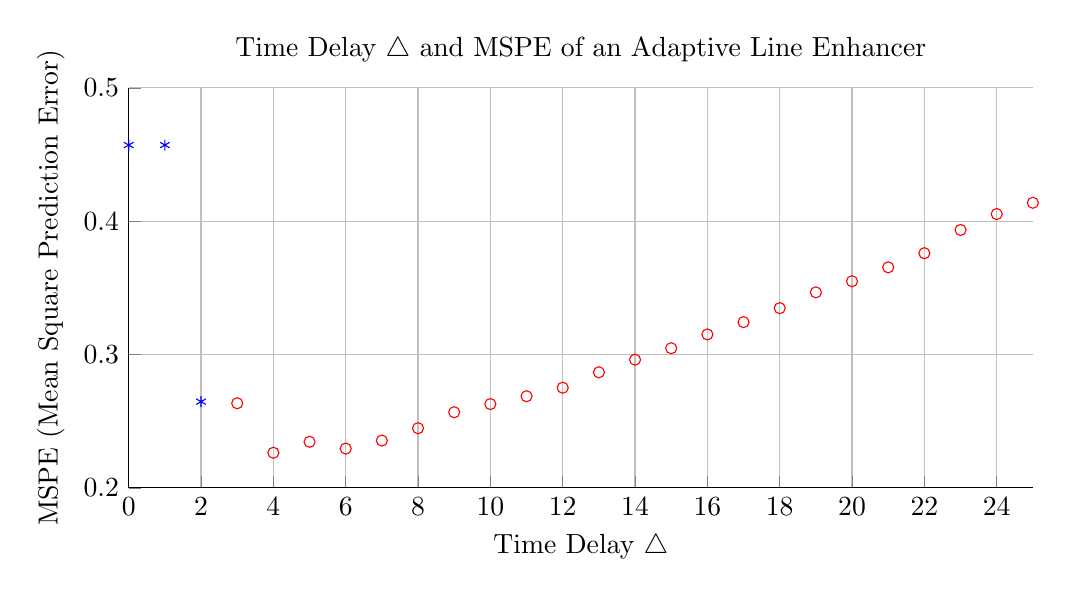
\begin{tikzpicture}

\begin{axis}[%
width=4.52083333333333in,
height=2in,
scale only axis,
xmin=0,
xmax=25,
xlabel={Time Delay $ \bigtriangleup $},
xmajorgrids,
ymin=0.2,
ymax=0.5,
ylabel={MSPE (Mean Square Prediction Error)},
ymajorgrids,
title={Time Delay $ \bigtriangleup $ and MSPE of an Adaptive Line Enhancer},
axis x line*=bottom,
axis y line*=left
]
\addplot [color=blue,only marks,mark=asterisk,mark options={solid},forget plot]
  table[row sep=crcr]{0	0.457112758906601\\
};
\addplot [color=blue,only marks,mark=asterisk,mark options={solid},forget plot]
  table[row sep=crcr]{1	0.457105598994501\\
};
\addplot [color=blue,only marks,mark=asterisk,mark options={solid},forget plot]
  table[row sep=crcr]{2	0.264648005573513\\
};
\addplot [color=red,only marks,mark=o,mark options={solid},forget plot]
  table[row sep=crcr]{3	0.263460490384655\\
};
\addplot [color=red,only marks,mark=o,mark options={solid},forget plot]
  table[row sep=crcr]{4	0.226349687179327\\
};
\addplot [color=red,only marks,mark=o,mark options={solid},forget plot]
  table[row sep=crcr]{5	0.234569847762656\\
};
\addplot [color=red,only marks,mark=o,mark options={solid},forget plot]
  table[row sep=crcr]{6	0.229458162435836\\
};
\addplot [color=red,only marks,mark=o,mark options={solid},forget plot]
  table[row sep=crcr]{7	0.235476978572889\\
};
\addplot [color=red,only marks,mark=o,mark options={solid},forget plot]
  table[row sep=crcr]{8	0.244740113347285\\
};
\addplot [color=red,only marks,mark=o,mark options={solid},forget plot]
  table[row sep=crcr]{9	0.256717932440133\\
};
\addplot [color=red,only marks,mark=o,mark options={solid},forget plot]
  table[row sep=crcr]{10	0.262847321334085\\
};
\addplot [color=red,only marks,mark=o,mark options={solid},forget plot]
  table[row sep=crcr]{11	0.268732331957349\\
};
\addplot [color=red,only marks,mark=o,mark options={solid},forget plot]
  table[row sep=crcr]{12	0.275114396677354\\
};
\addplot [color=red,only marks,mark=o,mark options={solid},forget plot]
  table[row sep=crcr]{13	0.28667927857361\\
};
\addplot [color=red,only marks,mark=o,mark options={solid},forget plot]
  table[row sep=crcr]{14	0.296155243031606\\
};
\addplot [color=red,only marks,mark=o,mark options={solid},forget plot]
  table[row sep=crcr]{15	0.304730148097582\\
};
\addplot [color=red,only marks,mark=o,mark options={solid},forget plot]
  table[row sep=crcr]{16	0.315095062870094\\
};
\addplot [color=red,only marks,mark=o,mark options={solid},forget plot]
  table[row sep=crcr]{17	0.324312346853434\\
};
\addplot [color=red,only marks,mark=o,mark options={solid},forget plot]
  table[row sep=crcr]{18	0.334793987827317\\
};
\addplot [color=red,only marks,mark=o,mark options={solid},forget plot]
  table[row sep=crcr]{19	0.346640873844623\\
};
\addplot [color=red,only marks,mark=o,mark options={solid},forget plot]
  table[row sep=crcr]{20	0.355001454398426\\
};
\addplot [color=red,only marks,mark=o,mark options={solid},forget plot]
  table[row sep=crcr]{21	0.365391974658412\\
};
\addplot [color=red,only marks,mark=o,mark options={solid},forget plot]
  table[row sep=crcr]{22	0.376014463963637\\
};
\addplot [color=red,only marks,mark=o,mark options={solid},forget plot]
  table[row sep=crcr]{23	0.393427558802103\\
};
\addplot [color=red,only marks,mark=o,mark options={solid},forget plot]
  table[row sep=crcr]{24	0.405385769010224\\
};
\addplot [color=red,only marks,mark=o,mark options={solid},forget plot]
  table[row sep=crcr]{25	0.413840200854496\\
};
\end{axis}
\end{tikzpicture}%}
		\caption{\textit{Differing delays plotted against their MSPEs}}
		\label{fig:3_3_b_delay}
	\end{subfigure}
	~ %add desired spacing between images, e. g. ~, \quad, \qquad, \hfill etc.
	%(or a blank line to force the subfigure onto a new line)
	\begin{subfigure}[b]{0.49\textwidth}
		\resizebox{\textwidth}{2in}{% This file was created by matlab2tikz v0.4.7 (commit 1fe4f59b3318f420f97af7fe257e27c8a5568af7) running on MATLAB 8.3.
% Copyright (c) 2008--2014, Nico Schlömer <nico.schloemer@gmail.com>
% All rights reserved.
% Minimal pgfplots version: 1.3
% 
% The latest updates can be retrieved from
%   http://www.mathworks.com/matlabcentral/fileexchange/22022-matlab2tikz
% where you can also make suggestions and rate matlab2tikz.
% 
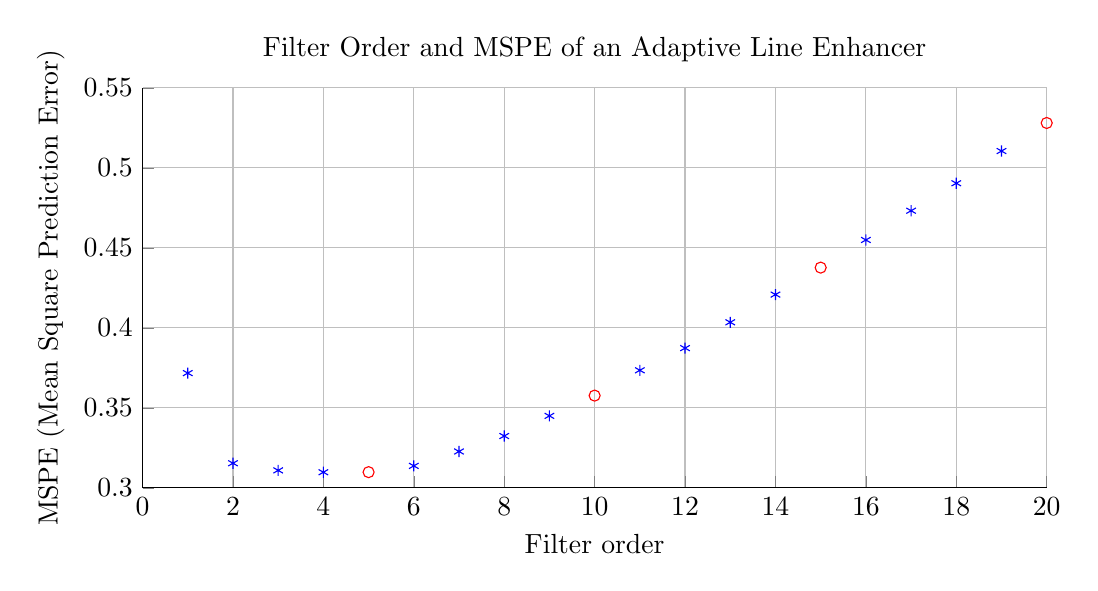
\begin{tikzpicture}

\begin{axis}[%
width=4.52083333333333in,
height=2in,
scale only axis,
xmin=0,
xmax=20,
xlabel={Filter order},
xmajorgrids,
ymin=0.3,
ymax=0.55,
ylabel={MSPE (Mean Square Prediction Error)},
ymajorgrids,
title={Filter Order and MSPE of an Adaptive Line Enhancer},
axis x line*=bottom,
axis y line*=left
]
\addplot [color=blue,only marks,mark=asterisk,mark options={solid},forget plot]
  table[row sep=crcr]{1	0.371726381800755\\
};
\addplot [color=blue,only marks,mark=asterisk,mark options={solid},forget plot]
  table[row sep=crcr]{2	0.315391042127382\\
};
\addplot [color=blue,only marks,mark=asterisk,mark options={solid},forget plot]
  table[row sep=crcr]{3	0.310931706311044\\
};
\addplot [color=blue,only marks,mark=asterisk,mark options={solid},forget plot]
  table[row sep=crcr]{4	0.309766821444037\\
};
\addplot [color=red,only marks,mark=o,mark options={solid},forget plot]
  table[row sep=crcr]{5	0.309828642561204\\
};
\addplot [color=blue,only marks,mark=asterisk,mark options={solid},forget plot]
  table[row sep=crcr]{6	0.313745036439469\\
};
\addplot [color=blue,only marks,mark=asterisk,mark options={solid},forget plot]
  table[row sep=crcr]{7	0.322740841685012\\
};
\addplot [color=blue,only marks,mark=asterisk,mark options={solid},forget plot]
  table[row sep=crcr]{8	0.332408214998103\\
};
\addplot [color=blue,only marks,mark=asterisk,mark options={solid},forget plot]
  table[row sep=crcr]{9	0.344997250858036\\
};
\addplot [color=red,only marks,mark=o,mark options={solid},forget plot]
  table[row sep=crcr]{10	0.357669285648671\\
};
\addplot [color=blue,only marks,mark=asterisk,mark options={solid},forget plot]
  table[row sep=crcr]{11	0.373487997313038\\
};
\addplot [color=blue,only marks,mark=asterisk,mark options={solid},forget plot]
  table[row sep=crcr]{12	0.387349352597067\\
};
\addplot [color=blue,only marks,mark=asterisk,mark options={solid},forget plot]
  table[row sep=crcr]{13	0.403487857286734\\
};
\addplot [color=blue,only marks,mark=asterisk,mark options={solid},forget plot]
  table[row sep=crcr]{14	0.420809083542202\\
};
\addplot [color=red,only marks,mark=o,mark options={solid},forget plot]
  table[row sep=crcr]{15	0.437662318060958\\
};
\addplot [color=blue,only marks,mark=asterisk,mark options={solid},forget plot]
  table[row sep=crcr]{16	0.454939357318857\\
};
\addplot [color=blue,only marks,mark=asterisk,mark options={solid},forget plot]
  table[row sep=crcr]{17	0.473212506157483\\
};
\addplot [color=blue,only marks,mark=asterisk,mark options={solid},forget plot]
  table[row sep=crcr]{18	0.490389962458254\\
};
\addplot [color=blue,only marks,mark=asterisk,mark options={solid},forget plot]
  table[row sep=crcr]{19	0.510532231200158\\
};
\addplot [color=red,only marks,mark=o,mark options={solid},forget plot]
  table[row sep=crcr]{20	0.528059996011193\\
};
\end{axis}
\end{tikzpicture}%}
		\caption{\textit{Differing filter orders plotted against their MSPEs}}
		\label{fig:3_3_b_order}
	\end{subfigure}
	
	\label{fig:3_3_b_sweeps}
	\caption{\textit{MSPE of the Adaptive Line Enhancer, with varying parameters of input delay and filter order}}
\end{figure}

Using the parameters $ \bigtriangleup = 4$ and $ M = 5$, we can produce a plot of the input signal without noise $x(n)$, once noise has been added, $s(n)$ and the new estimated output. As with other experiments, multiple iterations have been taken, and the mean sampled from these (as has been done in other parts of the coursework, as well). This is shown in figure \ref{fig:3_3_b_overview}. The delay on the output signal as created by $ \mathbf{u}(n) $ is apparent. We also observe that the amplitude of noise is noticeably smaller on the output than the input - so we know the ALE has had some effect to improve the signal.

\begin{figure}[h]
\centering 
\resizebox{\textwidth}{!}{% This file was created by matlab2tikz v0.4.7 (commit 84da6da3eee1f984abca8102d577f21df97f7554) running on MATLAB 8.3.
% Copyright (c) 2008--2014, Nico Schlömer <nico.schloemer@gmail.com>
% All rights reserved.
% Minimal pgfplots version: 1.3
% 
% The latest updates can be retrieved from
%   http://www.mathworks.com/matlabcentral/fileexchange/22022-matlab2tikz
% where you can also make suggestions and rate matlab2tikz.
% 
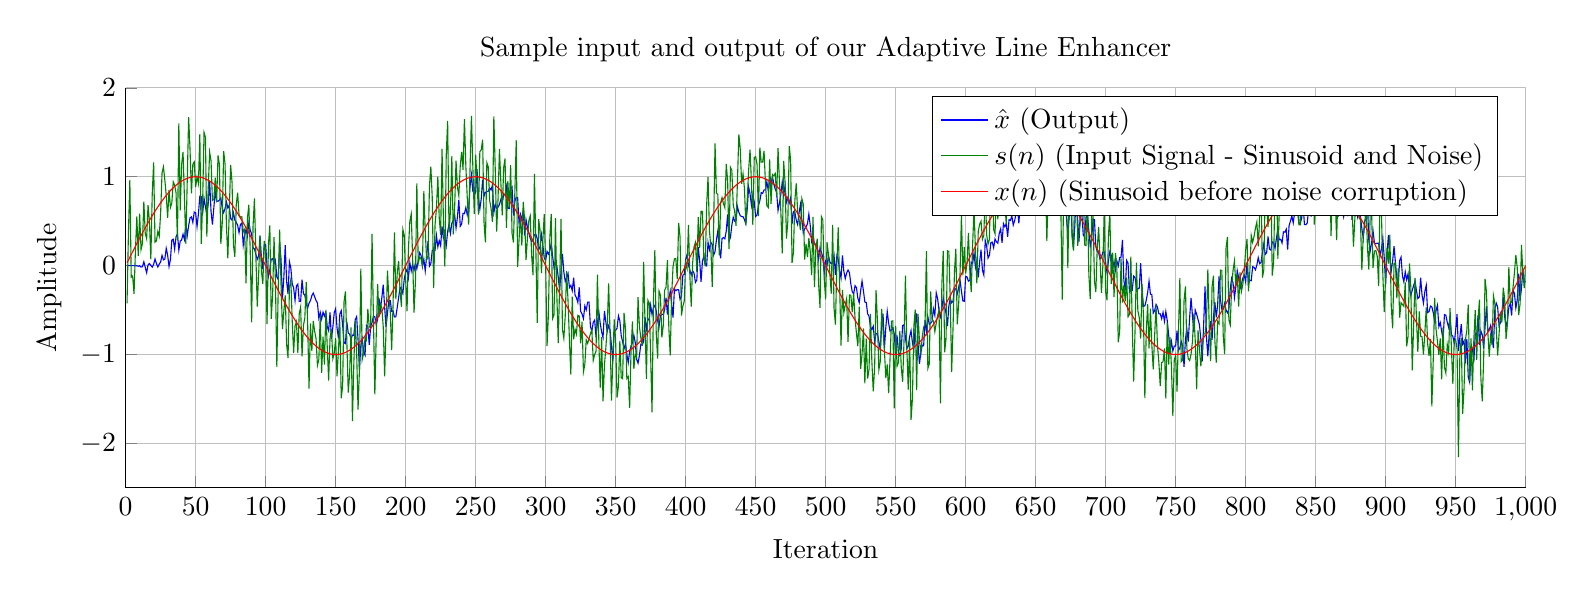
\begin{tikzpicture}

\begin{axis}[%
width=7in,
height=2in,scale only axis,
xmin=0,
xmax=1000,
xmajorgrids,
ymin=-2.5,
ymax=2,
xlabel={Iteration},
ylabel={Amplitude},
title={Sample input and output of our Adaptive Line Enhancer},
ymajorgrids,
axis x line*=bottom,
axis y line*=left,
legend style={draw=black,fill=white,legend cell align=left}
]
\addplot [color=blue,solid]
  table[row sep=crcr]{1	0\\
2	0\\
3	0\\
4	0\\
5	0\\
6	0\\
7	-0.00199102555916117\\
8	-0.000766145882907468\\
9	-0.00746507157746659\\
10	-0.0011438951318584\\
11	-0.0154885905415642\\
12	-0.0119387227500404\\
13	0.0427848745191654\\
14	-0.0192570699964584\\
15	-0.0795890699950323\\
16	0.00786769345781545\\
17	0.023256496239273\\
18	0.00258770401880402\\
19	-0.0161217301894514\\
20	0.0154240542528933\\
21	0.0741767899204495\\
22	0.0236578723521825\\
23	-0.0153577235663237\\
24	0.0181589102523915\\
25	0.0413544212909036\\
26	0.115308703485641\\
27	0.0647687153948198\\
28	0.0729800249888457\\
29	0.195631404085482\\
30	0.117527393203315\\
31	-0.0103303636097468\\
32	0.0691283937488014\\
33	0.288246744648575\\
34	0.297678253085652\\
35	0.184725620560943\\
36	0.325505429586181\\
37	0.356276183475806\\
38	0.174108371107518\\
39	0.275258756547219\\
40	0.289827651655907\\
41	0.353072460012318\\
42	0.29475452498717\\
43	0.473295512471967\\
44	0.336422258235427\\
45	0.4486193953677\\
46	0.537325529056692\\
47	0.548719739965506\\
48	0.485262466239149\\
49	0.60339231994558\\
50	0.594811699833565\\
51	0.439090958786233\\
52	0.583032457746278\\
53	0.781445091654959\\
54	0.776090382478886\\
55	0.583987350694774\\
56	0.757717025627791\\
57	0.66089315219505\\
58	0.573127301537733\\
59	0.700611399555099\\
60	0.954395158720876\\
61	0.610163317233044\\
62	0.46320599184687\\
63	0.65284970255461\\
64	0.833713529045415\\
65	0.729277017005349\\
66	0.723797255958874\\
67	0.738062863355618\\
68	0.76125907018666\\
69	0.645643724799343\\
70	0.594871924451171\\
71	0.644224672652132\\
72	0.717826634272784\\
73	0.649442226389299\\
74	0.679789933621623\\
75	0.529916362507892\\
76	0.511954843911147\\
77	0.594251012830241\\
78	0.511995285313465\\
79	0.489167592018595\\
80	0.454437434589745\\
81	0.371417072000321\\
82	0.463757610003286\\
83	0.479905517769415\\
84	0.230022877165632\\
85	0.339679479425045\\
86	0.410299481245618\\
87	0.332983059686399\\
88	0.482204801938636\\
89	0.399232411611278\\
90	0.356510112323953\\
91	0.200831136936811\\
92	0.188901872802032\\
93	0.12799976008288\\
94	0.0715280421195802\\
95	0.109104165057473\\
96	0.330129532151706\\
97	0.087886638218369\\
98	-0.0402140685563188\\
99	0.233984105806403\\
100	0.238571587526379\\
101	-0.00712391575812748\\
102	-0.121725570713935\\
103	-0.0421359505776701\\
104	0.0721021284380138\\
105	0.0790808014608243\\
106	0.0228648269417988\\
107	0.0596582485182969\\
108	-0.129044773271046\\
109	-0.156246468411231\\
110	0.245533689421426\\
111	0.0729271528200256\\
112	-0.373789756691909\\
113	-0.133404140161232\\
114	0.230089680805427\\
115	-0.180522213818034\\
116	-0.320297263558827\\
117	0.043499661175\\
118	-0.0284688806199213\\
119	-0.205313909296677\\
120	-0.248806224141722\\
121	-0.392368936303206\\
122	-0.227000090127444\\
123	-0.207340854208872\\
124	-0.402654089521316\\
125	-0.40240137412925\\
126	-0.157930901252966\\
127	-0.315094696862124\\
128	-0.331815752510444\\
129	-0.430348745202688\\
130	-0.478492811124092\\
131	-0.42174434466586\\
132	-0.393857416262089\\
133	-0.337984834078626\\
134	-0.308115565830087\\
135	-0.349620542805586\\
136	-0.391258151338648\\
137	-0.419447048129861\\
138	-0.591499675658761\\
139	-0.52517807466556\\
140	-0.60264578453679\\
141	-0.523053723564664\\
142	-0.5673475877239\\
143	-0.518891705652115\\
144	-0.684367017925629\\
145	-0.73258333092744\\
146	-0.527271532031338\\
147	-0.823431720565026\\
148	-0.695293901852767\\
149	-0.528776053524467\\
150	-0.484836006505405\\
151	-0.700898330332902\\
152	-0.817334745806778\\
153	-0.544483926674373\\
154	-0.506497048568432\\
155	-0.671957810161982\\
156	-0.868199455252385\\
157	-0.87735611301354\\
158	-0.631896515854211\\
159	-0.758065894464125\\
160	-0.770219225916565\\
161	-0.829433687399374\\
162	-0.781007685022397\\
163	-0.784024982298875\\
164	-0.606901053895351\\
165	-0.574114525429896\\
166	-0.83051928679249\\
167	-1.17014313515529\\
168	-0.89853452597676\\
169	-0.821744612880942\\
170	-0.967775824123561\\
171	-1.00696999533092\\
172	-0.670198941477381\\
173	-0.681618196665026\\
174	-0.890172808220678\\
175	-0.687949231399095\\
176	-0.638809861748195\\
177	-0.568049540422856\\
178	-0.574871343901212\\
179	-0.66326702734244\\
180	-0.600427210141353\\
181	-0.368525988729571\\
182	-0.492231132401869\\
183	-0.360673872270485\\
184	-0.214366458977919\\
185	-0.469406156291556\\
186	-0.69164247852806\\
187	-0.538959479437831\\
188	-0.39488740991298\\
189	-0.39138330761625\\
190	-0.514838527599459\\
191	-0.507982922507557\\
192	-0.577053146596337\\
193	-0.575441798089245\\
194	-0.469040743077728\\
195	-0.358150217328688\\
196	-0.244461434386716\\
197	-0.264932107374394\\
198	-0.311823858157541\\
199	-0.151802870244204\\
200	-0.0751878134568607\\
201	-0.0415194429327213\\
202	-0.136293714143652\\
203	0.0315468495961406\\
204	-0.0597236087241191\\
205	0.0143942041844737\\
206	-0.0517733023346956\\
207	0.0347448877138816\\
208	-0.0339515496309887\\
209	0.0562640907506905\\
210	0.146036095288093\\
211	0.114899860178801\\
212	-0.00632079525813114\\
213	0.0724834218515131\\
214	-0.0587118197103165\\
215	0.113275748495006\\
216	0.274509719263564\\
217	-0.00649131575053957\\
218	0.020414537906754\\
219	0.169370634995857\\
220	0.178955426803328\\
221	0.173989840470099\\
222	0.339376174007709\\
223	0.211727624335497\\
224	0.280513576388861\\
225	0.224527573132391\\
226	0.441410186285325\\
227	0.305591694716159\\
228	0.316907509979059\\
229	0.22231777206933\\
230	0.384724455383279\\
231	0.468193607347647\\
232	0.363511277068078\\
233	0.477672862735045\\
234	0.508889582088084\\
235	0.573018873942862\\
236	0.422938002004728\\
237	0.544661769811037\\
238	0.740784589037536\\
239	0.442967489184726\\
240	0.468455010792239\\
241	0.588730295810935\\
242	0.585351526136105\\
243	0.653894054337933\\
244	0.570580082134261\\
245	0.628413696229843\\
246	0.888821156995639\\
247	1.02227887169124\\
248	0.835622854241739\\
249	0.844418672085988\\
250	0.820536504045253\\
251	1.08558641739313\\
252	0.764133610294103\\
253	0.636975395635685\\
254	0.751289888888468\\
255	0.967665185404839\\
256	0.782097355985514\\
257	0.825554457273151\\
258	0.830464518728401\\
259	0.838286079147512\\
260	0.874132212185337\\
261	0.85054445889643\\
262	0.908293121878117\\
263	0.597687204437049\\
264	0.687695591209216\\
265	0.645758597196062\\
266	0.65797899415303\\
267	0.687586834697373\\
268	0.74462883961226\\
269	0.711633574805476\\
270	0.799447902407673\\
271	0.798169667572516\\
272	0.885593305776175\\
273	0.645586152085587\\
274	0.64253341080377\\
275	0.870122319027895\\
276	0.887034679232992\\
277	0.563046444724339\\
278	0.725374479443217\\
279	0.767921591330992\\
280	0.765783998041802\\
281	0.479582771055795\\
282	0.575853194022398\\
283	0.512613713766684\\
284	0.622634111005594\\
285	0.338158102994802\\
286	0.517402884032394\\
287	0.432870571507242\\
288	0.368588142130721\\
289	0.308058032368157\\
290	0.268595795433584\\
291	0.287284057193325\\
292	0.351812497392528\\
293	0.35319690312359\\
294	0.30418837760709\\
295	0.17804981473016\\
296	0.215541089566079\\
297	0.35094644048072\\
298	0.234113704657299\\
299	0.085657463474028\\
300	0.0587583329129236\\
301	0.15954613178189\\
302	0.129425347105563\\
303	0.170670212273769\\
304	0.250105487610964\\
305	0.10366172460957\\
306	-0.0254185642499514\\
307	0.0141130290749601\\
308	-0.00172781161391359\\
309	-0.128926989557269\\
310	-0.280796981383286\\
311	-0.059837710702124\\
312	0.130887440007101\\
313	-0.0718456079849847\\
314	-0.177939180036077\\
315	-0.13463759374473\\
316	-0.0876203928253484\\
317	-0.246604559268779\\
318	-0.221666694150721\\
319	-0.2808068543461\\
320	-0.135089152569774\\
321	-0.330653329103797\\
322	-0.361281212682688\\
323	-0.413939760998332\\
324	-0.243496751806242\\
325	-0.513976667378442\\
326	-0.543446225119378\\
327	-0.596138854013329\\
328	-0.452917981459305\\
329	-0.49813461586275\\
330	-0.411727853901771\\
331	-0.410036985301103\\
332	-0.684412769978712\\
333	-0.738640774960936\\
334	-0.637282193575891\\
335	-0.612647826160882\\
336	-0.805358379523656\\
337	-0.647225767121241\\
338	-0.517555392873169\\
339	-0.650125097911366\\
340	-0.746173258091948\\
341	-0.808747166942455\\
342	-0.509921288260603\\
343	-0.634078091390086\\
344	-0.738214631197746\\
345	-0.674574072493591\\
346	-0.723973478503672\\
347	-0.897834620627897\\
348	-1.07475112352434\\
349	-0.735793730385978\\
350	-0.727017554290359\\
351	-0.704483209668839\\
352	-0.564623841168548\\
353	-0.619457209368478\\
354	-0.788602483239912\\
355	-0.857444858944427\\
356	-0.93527955363334\\
357	-0.877695610428705\\
358	-0.996771907238217\\
359	-1.09218954295941\\
360	-0.966170499869425\\
361	-0.905083602996474\\
362	-0.866854969317629\\
363	-0.782337562982962\\
364	-0.864610060478855\\
365	-1.0550596266113\\
366	-1.09685479340009\\
367	-1.00867862120585\\
368	-0.884690270358512\\
369	-0.893433986426244\\
370	-0.850468062677266\\
371	-0.578889571122568\\
372	-0.70963382294108\\
373	-0.613396515458933\\
374	-0.594591822199573\\
375	-0.444270736032323\\
376	-0.550983717223735\\
377	-0.471495467178712\\
378	-0.447166779813082\\
379	-0.507903203582954\\
380	-0.618406938910878\\
381	-0.68938740858919\\
382	-0.561346141770375\\
383	-0.549512326984542\\
384	-0.546664052368475\\
385	-0.496709176143666\\
386	-0.359030495749815\\
387	-0.549426472808549\\
388	-0.375184858493267\\
389	-0.28716501836068\\
390	-0.435932828061277\\
391	-0.583101044627079\\
392	-0.259108891009325\\
393	-0.282295564486655\\
394	-0.269460325890878\\
395	-0.271761154086517\\
396	-0.379099838380413\\
397	-0.34512737424831\\
398	-0.107976868689703\\
399	-0.0968680969950371\\
400	0.0656680784270037\\
401	0.123378954527845\\
402	0.0066477359265674\\
403	-0.0500642051548049\\
404	-0.104988769160406\\
405	-0.056504104734372\\
406	-0.0855147904170734\\
407	-0.187912192138168\\
408	-0.16070822285105\\
409	0.207202006925674\\
410	0.0601361937648822\\
411	-0.182806209289777\\
412	0.0511405354349759\\
413	0.106486818116199\\
414	0.0165692864928624\\
415	-0.00133571325263244\\
416	0.260565648724987\\
417	0.179253617500881\\
418	0.263063897317437\\
419	0.236817552819522\\
420	0.119180164589013\\
421	0.158450770801204\\
422	0.292500752299489\\
423	0.389546710943932\\
424	0.207821817272297\\
425	0.0834275197642773\\
426	0.305623477211353\\
427	0.315555011813986\\
428	0.302196355405004\\
429	0.387762319209013\\
430	0.577463971192993\\
431	0.275153633463174\\
432	0.317149445327249\\
433	0.457117378313831\\
434	0.544429409251146\\
435	0.502369261277569\\
436	0.512635033470477\\
437	0.663687018294557\\
438	0.601577280647234\\
439	0.562515986095\\
440	0.551860570022385\\
441	0.55119211540348\\
442	0.517920545010311\\
443	0.46845380385669\\
444	0.640555398168316\\
445	0.886396023210865\\
446	0.80776206985098\\
447	0.677436501254152\\
448	0.789446001010086\\
449	0.71867989255955\\
450	0.552688622517635\\
451	0.568721454367775\\
452	0.677177739523173\\
453	0.729665015868632\\
454	0.82209401366659\\
455	0.812872868008719\\
456	0.852254398343493\\
457	0.851572471976841\\
458	0.944339148754235\\
459	0.846067567227073\\
460	0.961314472850341\\
461	0.914460146699515\\
462	1.00574951556814\\
463	0.915990540870483\\
464	0.860553592516989\\
465	0.823867524102249\\
466	0.620745378240824\\
467	0.701894587878513\\
468	0.802710082468311\\
469	0.938781464701199\\
470	0.787550551782153\\
471	0.897724919384353\\
472	0.712930415935413\\
473	0.764675375572766\\
474	0.703476705635358\\
475	0.76434300801301\\
476	0.468482341561279\\
477	0.609409290257679\\
478	0.602018348412824\\
479	0.510962781242846\\
480	0.463623716548092\\
481	0.592780977338654\\
482	0.688936625655779\\
483	0.518316810667209\\
484	0.370126810582715\\
485	0.411927431985336\\
486	0.438219886221085\\
487	0.469811088415032\\
488	0.5806449094928\\
489	0.451558254738308\\
490	0.274094650115529\\
491	0.338033704744004\\
492	0.244320284728647\\
493	0.244105508315932\\
494	0.176438554731368\\
495	0.0711692884294946\\
496	0.201595771288908\\
497	0.149194329739061\\
498	0.0930153847110273\\
499	-0.0904581561665942\\
500	0.0462473409814707\\
501	0.00243231409182619\\
502	0.114399428828972\\
503	0.0421427061319619\\
504	0.019999799728057\\
505	0.0393500868926022\\
506	0.116778291288801\\
507	-0.102703278034316\\
508	0.108191283320782\\
509	0.0711463471184554\\
510	-0.0583927911514153\\
511	-0.138411665140961\\
512	0.114723948234123\\
513	-0.0636077199611603\\
514	-0.144806198236795\\
515	-0.082302830751844\\
516	-0.0491618935989711\\
517	-0.0785773038962827\\
518	-0.206492958989052\\
519	-0.292155836962093\\
520	-0.319875873147297\\
521	-0.226072428408524\\
522	-0.246163421450734\\
523	-0.36559736780492\\
524	-0.415974776356222\\
525	-0.280479210121231\\
526	-0.174060315075046\\
527	-0.283610445731984\\
528	-0.408521118754063\\
529	-0.415559205265358\\
530	-0.542158623159627\\
531	-0.569549441717858\\
532	-0.686771361393827\\
533	-0.719450532136873\\
534	-0.681018841134337\\
535	-0.858430273996841\\
536	-0.76764159018292\\
537	-0.760876739723188\\
538	-0.85243717020472\\
539	-0.939225269606256\\
540	-0.68183679080709\\
541	-0.540831247224229\\
542	-0.930222363230104\\
543	-0.688617081636441\\
544	-0.514206393411139\\
545	-0.647608962214666\\
546	-0.735890660563445\\
547	-0.724503190941864\\
548	-0.698477985512945\\
549	-0.767517292937004\\
550	-0.996437817874938\\
551	-0.783510635697308\\
552	-0.978419414324571\\
553	-1.00833669069883\\
554	-0.936812524870027\\
555	-0.673253419584233\\
556	-0.665144350056322\\
557	-0.810939254803533\\
558	-0.931302614239998\\
559	-0.905789298987268\\
560	-0.798880234691247\\
561	-0.730421293142736\\
562	-0.866168926706018\\
563	-0.950598074764708\\
564	-0.67414246319161\\
565	-0.537286405849674\\
566	-0.877180670290969\\
567	-1.10564992168977\\
568	-0.98017194722291\\
569	-0.893992244369497\\
570	-0.900662866841995\\
571	-0.614009127581355\\
572	-0.736761146588911\\
573	-0.573851455303102\\
574	-0.659683419935141\\
575	-0.647154629196257\\
576	-0.628609701180642\\
577	-0.48737557023241\\
578	-0.558577548185908\\
579	-0.305171980604269\\
580	-0.372247154232022\\
581	-0.507789278519077\\
582	-0.575594296029879\\
583	-0.485771513518578\\
584	-0.360367673644097\\
585	-0.458682615801247\\
586	-0.537955411250679\\
587	-0.681102456027208\\
588	-0.454306829009057\\
589	-0.36612167462459\\
590	-0.418011187270798\\
591	-0.396979970924195\\
592	-0.252721542690874\\
593	-0.26543066708976\\
594	-0.31755101217708\\
595	-0.246164188901291\\
596	-0.165035481603622\\
597	-0.288377727332005\\
598	-0.397502200335717\\
599	-0.399867714932617\\
600	-0.120324634823389\\
601	-0.126483412351469\\
602	-0.174190015036516\\
603	-0.165114857151143\\
604	0.038374635782764\\
605	0.021633326667722\\
606	0.143960705813444\\
607	-0.0202628148832196\\
608	0.0492281207959032\\
609	-0.131538948472118\\
610	0.042957395595262\\
611	0.178631135839994\\
612	-0.0538192412685167\\
613	-0.106622260083159\\
614	0.284615090178936\\
615	0.220470049374929\\
616	0.0855829121308054\\
617	0.116404824932886\\
618	0.258395510924905\\
619	0.264732452865226\\
620	0.201171530161955\\
621	0.300970823973181\\
622	0.269208389215355\\
623	0.253348931691705\\
624	0.362702321076204\\
625	0.413415825771745\\
626	0.256798848563139\\
627	0.473676311777122\\
628	0.438173738865381\\
629	0.472448593919163\\
630	0.325365969256883\\
631	0.516992317598702\\
632	0.509205328920079\\
633	0.560367025984597\\
634	0.457196894071505\\
635	0.505456750011886\\
636	0.587429913805485\\
637	0.667763825689915\\
638	0.476137721155842\\
639	0.699533818823247\\
640	0.748007584254939\\
641	0.698359313916181\\
642	0.753361824684729\\
643	0.863297936712952\\
644	0.825521624563509\\
645	0.828572131882284\\
646	0.930326164425059\\
647	0.868999474154728\\
648	0.731012409283273\\
649	0.699841280224803\\
650	0.960713168986389\\
651	0.858781228993183\\
652	0.922925454043379\\
653	0.887276824618533\\
654	1.01403401741196\\
655	1.03900275138355\\
656	1.0464059306483\\
657	0.813140701824668\\
658	1.05604016923932\\
659	0.897655626401414\\
660	0.976934512452778\\
661	0.981431757172901\\
662	0.995440399376633\\
663	0.759587516852996\\
664	0.82091366272288\\
665	0.662986120074669\\
666	0.677590178144137\\
667	0.823458293893591\\
668	0.788473526323766\\
669	0.795244476114903\\
670	0.670389719008407\\
671	0.75612612476921\\
672	0.53409996605293\\
673	0.354427733822164\\
674	0.55514369778572\\
675	0.80651487763047\\
676	0.373256930288757\\
677	0.194916368161515\\
678	0.450986354417442\\
679	0.84643763771304\\
680	0.521070341725461\\
681	0.269980770037821\\
682	0.668203223835273\\
683	0.58591427065513\\
684	0.347236746463386\\
685	0.317420557259548\\
686	0.549029288546824\\
687	0.575336250348126\\
688	0.396212264337268\\
689	0.21669046228287\\
690	0.298816642097809\\
691	0.524037483791077\\
692	0.516954879407573\\
693	0.214289578767656\\
694	0.157482208459045\\
695	0.142253262809177\\
696	0.0773606406633782\\
697	0.0948309113603279\\
698	0.151938531829854\\
699	0.154602960996568\\
700	0.0335819464976309\\
701	-0.082511757476297\\
702	0.0518576966271238\\
703	0.159263390991608\\
704	0.116531899896819\\
705	-0.0359911212821424\\
706	0.0475066009836978\\
707	-0.0504572126284515\\
708	0.0541640322983626\\
709	-0.00299945655368837\\
710	0.0912041440823129\\
711	0.0955976196810132\\
712	0.288987152486399\\
713	-0.163085650390442\\
714	-0.276956928009826\\
715	0.0593225594172983\\
716	0.0281880318089265\\
717	-0.295293526698778\\
718	-0.279900085030065\\
719	-0.276996627411763\\
720	-0.117343049111174\\
721	-0.133876373619919\\
722	-0.248721819971272\\
723	-0.263546414983977\\
724	-0.252914408349178\\
725	0.0270754661287338\\
726	-0.289704125591452\\
727	-0.457369972378739\\
728	-0.452717513419435\\
729	-0.390067822861302\\
730	-0.303776868289222\\
731	-0.17361082717363\\
732	-0.320987727241119\\
733	-0.325659161424245\\
734	-0.533736630399667\\
735	-0.505330252711621\\
736	-0.43655444183859\\
737	-0.465290466418301\\
738	-0.542618691423572\\
739	-0.54181721725745\\
740	-0.596591204089425\\
741	-0.525668438391159\\
742	-0.625829192130081\\
743	-0.515452160578246\\
744	-0.618474015514007\\
745	-0.777813069984126\\
746	-0.959369902248443\\
747	-0.853749238202037\\
748	-0.959453515389805\\
749	-0.904444937293889\\
750	-0.905297236321374\\
751	-0.73243246932108\\
752	-0.953436057884067\\
753	-0.926631763152217\\
754	-0.853138901748263\\
755	-0.910908075309327\\
756	-1.13713887227306\\
757	-0.82430964212707\\
758	-0.71385894103636\\
759	-0.853975993909793\\
760	-0.585050198150118\\
761	-0.36173366279202\\
762	-0.562933152845267\\
763	-0.748814064434993\\
764	-0.499612205876927\\
765	-0.545688252729471\\
766	-0.606190011815717\\
767	-0.664632209085201\\
768	-0.829732521819559\\
769	-1.07575509369564\\
770	-0.662955628890862\\
771	-0.233407399490081\\
772	-0.801541498947696\\
773	-1.01958270481412\\
774	-0.746704717129217\\
775	-0.622624705962925\\
776	-0.834965989471901\\
777	-0.58115812596501\\
778	-0.407807506681795\\
779	-0.582099898802366\\
780	-0.439321958175742\\
781	-0.121321786615296\\
782	-0.382998029815396\\
783	-0.493561001062488\\
784	-0.488921460613771\\
785	-0.424737444192607\\
786	-0.498881805044086\\
787	-0.531284984777085\\
788	-0.494354877913889\\
789	-0.259940514856308\\
790	-0.141333699742312\\
791	-0.193705022751361\\
792	-0.359922170884638\\
793	-0.235301107894968\\
794	-0.0554700553007867\\
795	-0.136847536010948\\
796	-0.25957950494245\\
797	-0.209089160445904\\
798	-0.137340052282329\\
799	-0.108031950890353\\
800	-0.183571602832609\\
801	0.0345222393970454\\
802	-0.204691537245422\\
803	-0.162740405863088\\
804	-0.16891309756919\\
805	-0.0117157668425073\\
806	-0.019443602141569\\
807	-0.0469732701052909\\
808	0.00766668005361047\\
809	0.0891721022406494\\
810	0.0221289884494186\\
811	0.0360489560934018\\
812	0.150284932689253\\
813	0.246637465657177\\
814	0.125607776344707\\
815	0.145597027044416\\
816	0.327842952818542\\
817	0.185830760994969\\
818	0.176021372762237\\
819	0.266668507218223\\
820	0.254374212817331\\
821	0.194737126804811\\
822	0.309616815857374\\
823	0.407558057241483\\
824	0.290334841860807\\
825	0.296390768691957\\
826	0.254622209987569\\
827	0.380647712580395\\
828	0.37667226701872\\
829	0.410427216532974\\
830	0.179707833673789\\
831	0.447475279066467\\
832	0.501910726105839\\
833	0.557585776740438\\
834	0.48061607021884\\
835	0.602450553970872\\
836	0.813385830842534\\
837	0.630008759419513\\
838	0.475018927903791\\
839	0.473894932036867\\
840	0.534999172503444\\
841	0.696308714726114\\
842	0.462296813426216\\
843	0.460724590836661\\
844	0.480418724533285\\
845	0.63782810900014\\
846	0.568077627425784\\
847	0.560033495652515\\
848	0.623742011005992\\
849	0.732933663016339\\
850	0.88201283166078\\
851	0.771988010357052\\
852	0.655581605838023\\
853	0.657921441233799\\
854	0.70646217617484\\
855	0.76003552264541\\
856	0.618853974997347\\
857	0.778218394825194\\
858	0.857638822202932\\
859	0.697750775813767\\
860	0.846923431003603\\
861	0.738640806031863\\
862	0.618345934354791\\
863	0.698667582994944\\
864	0.779150064446034\\
865	0.672169878979035\\
866	0.549770167211897\\
867	0.768460662261341\\
868	0.635257006425918\\
869	0.635261081460224\\
870	0.549372002020791\\
871	0.642003777545501\\
872	0.627451087211883\\
873	0.571839776667211\\
874	0.628314408714937\\
875	0.778428489369243\\
876	0.51672755511032\\
877	0.63791534705764\\
878	0.780323258044938\\
879	0.618509742185429\\
880	0.546600122568475\\
881	0.720290252272727\\
882	0.550337940753062\\
883	0.41814163479945\\
884	0.307919725060038\\
885	0.499853184886134\\
886	0.520161135996128\\
887	0.714013729010765\\
888	0.273439604143174\\
889	0.167949750202472\\
890	0.261492511356607\\
891	0.391199064485752\\
892	0.253830600318006\\
893	0.247878781797958\\
894	0.251615158890257\\
895	0.25181007506588\\
896	0.106447974254638\\
897	0.191537642996201\\
898	0.308134473863821\\
899	0.0864761964741605\\
900	-0.212335870349549\\
901	0.144792311843977\\
902	0.343850153042645\\
903	0.0874436911936712\\
904	-0.0582373325893029\\
905	0.0523869911171848\\
906	0.219846924345201\\
907	0.0321155404300482\\
908	-0.14657955965604\\
909	-0.203899963961539\\
910	0.058104426519743\\
911	0.0957069903786524\\
912	-0.116395707594971\\
913	-0.182131548885477\\
914	-0.0698067808786876\\
915	-0.159217908198166\\
916	-0.0932911941499725\\
917	-0.261705243428127\\
918	-0.333441445756158\\
919	-0.276628616315482\\
920	-0.223894189729996\\
921	-0.173097896314471\\
922	-0.281223499739776\\
923	-0.36936175857865\\
924	-0.353686744093762\\
925	-0.136332332753186\\
926	-0.332415818174261\\
927	-0.421428902956695\\
928	-0.291429461154243\\
929	-0.220023869971373\\
930	-0.527707285851167\\
931	-0.517304824552557\\
932	-0.454910662834024\\
933	-0.464025213187917\\
934	-0.527426994313544\\
935	-0.629915628432878\\
936	-0.504289449497797\\
937	-0.446299450125169\\
938	-0.686613457567941\\
939	-0.640749747162455\\
940	-0.73606064590141\\
941	-0.835045253009571\\
942	-0.55102052178241\\
943	-0.556700875934844\\
944	-0.636522288560826\\
945	-0.69618817118419\\
946	-0.585258433286389\\
947	-0.776568227000704\\
948	-0.795130123880258\\
949	-0.8749490313022\\
950	-0.72538979022555\\
951	-0.546534024143478\\
952	-0.95949055854218\\
953	-0.806773839978851\\
954	-0.658447237634441\\
955	-0.882294722186273\\
956	-0.8472795136424\\
957	-1.09960758876109\\
958	-0.823554887038721\\
959	-1.25449561797781\\
960	-1.3109658107262\\
961	-0.982013912659969\\
962	-0.936841995574156\\
963	-1.08442368337181\\
964	-0.761168670696694\\
965	-0.78815276695812\\
966	-0.558505364815048\\
967	-0.891480867181614\\
968	-0.735170635027955\\
969	-0.777118541926563\\
970	-0.931898160525119\\
971	-0.696384985808778\\
972	-0.459295966989059\\
973	-0.735923096373303\\
974	-0.720970197296635\\
975	-0.672050783200447\\
976	-0.818306481338229\\
977	-0.926069512178673\\
978	-0.485227519455165\\
979	-0.421864845520357\\
980	-0.465386574008653\\
981	-0.676802914271864\\
982	-0.641088413819985\\
983	-0.570233732612348\\
984	-0.351783722520798\\
985	-0.573459652453132\\
986	-0.685172362682408\\
987	-0.621152196536119\\
988	-0.466266834201544\\
989	-0.426791733081662\\
990	-0.560337675028176\\
991	-0.277681528398188\\
992	-0.31117473232686\\
993	-0.476644912483058\\
994	-0.383852245574027\\
995	-0.0910706573695292\\
996	-0.394310054693832\\
997	-0.258071277197008\\
998	-0.0556112200482027\\
999	-0.167015569292188\\
1000	-0.188205930522682\\
};
\addlegendentry{$\hat{x} $ (Output)};

\addplot [color=black!50!green,solid]
  table[row sep=crcr]{1	-0.422987193463623\\
2	0.367665295400333\\
3	0.965701131608576\\
4	-0.129739517872119\\
5	-0.115756597763504\\
6	-0.318080634054704\\
7	0.171443172050897\\
8	0.552909786823387\\
9	0.111598328006877\\
10	0.585172478092126\\
11	0.180407773957908\\
12	0.248481598724005\\
13	0.720290543914178\\
14	0.364834339771426\\
15	0.303044839446141\\
16	0.681434667592683\\
17	0.498765983751313\\
18	0.0705187899926028\\
19	0.80599282656278\\
20	1.1605451352666\\
21	0.264509259341783\\
22	0.278839546134067\\
23	0.384842278968897\\
24	0.329234149242289\\
25	0.592380974530917\\
26	1.04266235564082\\
27	1.11150508453433\\
28	0.962973800048397\\
29	0.791665256249454\\
30	0.538802568969212\\
31	0.851516990894421\\
32	0.654901207240331\\
33	0.705727595373498\\
34	0.942881967907602\\
35	0.905711875996249\\
36	0.822377881097996\\
37	0.286515580635601\\
38	1.5995553908388\\
39	0.622101558895313\\
40	1.13976177146611\\
41	1.28017937434728\\
42	0.765444266226589\\
43	0.245896849588697\\
44	0.950337723559462\\
45	1.671230422797\\
46	1.30925977089156\\
47	0.812526499650889\\
48	1.1401484866779\\
49	1.16712254591277\\
50	0.884858138857317\\
51	0.998148714578203\\
52	0.924258007281299\\
53	1.48029214930006\\
54	0.244786350119877\\
55	0.707029148721094\\
56	1.49923840198319\\
57	1.44414769644842\\
58	0.327491801735904\\
59	0.879859929945525\\
60	1.27625363347311\\
61	1.18089698055207\\
62	0.733306237605915\\
63	0.747158753978446\\
64	0.988858358024128\\
65	0.711328950711561\\
66	1.24036725621636\\
67	1.13822969121274\\
68	0.244558955676161\\
69	0.47780309393082\\
70	1.28826189022248\\
71	1.14785671526541\\
72	0.452233252453422\\
73	0.0823629896023944\\
74	0.594617640912281\\
75	1.13373285125953\\
76	0.939265341847842\\
77	0.237809823806049\\
78	0.0987649162978081\\
79	0.683364588037961\\
80	0.822061485773898\\
81	0.570749652164912\\
82	0.545273922186052\\
83	0.550365301731108\\
84	0.380017252672683\\
85	0.409131323524026\\
86	-0.199397356701494\\
87	0.534729524181391\\
88	0.684851379326422\\
89	0.16040829036547\\
90	-0.636844677184856\\
91	0.439731734647471\\
92	0.757358667880901\\
93	0.132325345931298\\
94	-0.460528420491904\\
95	-0.104555958441868\\
96	0.339442071441078\\
97	-0.0654487223107544\\
98	-0.204792376607681\\
99	0.278542764399076\\
100	0.156866451134759\\
101	-0.656359603506427\\
102	0.233916013306119\\
103	0.453337247507035\\
104	-0.599446827753515\\
105	-0.325164935289312\\
106	0.32085592119047\\
107	-0.180753102705497\\
108	-1.13973475251768\\
109	-0.24528789715668\\
110	0.405018602047061\\
111	-0.212468306552941\\
112	-0.714445167388089\\
113	-0.514700678815686\\
114	-0.334462702386076\\
115	-0.885683032242607\\
116	-1.0388771617616\\
117	-0.246031797735541\\
118	-0.155762425041052\\
119	-0.625931120910387\\
120	-0.98309170268418\\
121	-0.678181462747527\\
122	-0.631932032784189\\
123	-0.982629058212951\\
124	-0.54190253403403\\
125	-0.464816465046983\\
126	-1.0200543260868\\
127	-0.673600582543542\\
128	-0.587457594873718\\
129	-0.186413333390882\\
130	-0.641222368030653\\
131	-1.38228795654353\\
132	-0.650843193454837\\
133	-0.958980592508669\\
134	-0.622691750618276\\
135	-0.735838198850659\\
136	-0.820760873025134\\
137	-1.12308594072249\\
138	-1.05527748392793\\
139	-0.560847875241884\\
140	-1.20694349848098\\
141	-0.799655067137348\\
142	-1.1139870593661\\
143	-0.505728902065666\\
144	-0.911592042961856\\
145	-1.29248658711922\\
146	-0.817502839006449\\
147	-0.710786842879045\\
148	-1.04590049448486\\
149	-0.984787965109705\\
150	-0.816191675931922\\
151	-1.24449307941313\\
152	-0.947624715048146\\
153	-0.629491356423615\\
154	-1.49124059522242\\
155	-1.35292903671298\\
156	-0.406378737122216\\
157	-0.291065727325327\\
158	-0.846679218226706\\
159	-1.42769613779046\\
160	-1.22041887572966\\
161	-0.695105329571839\\
162	-1.74948672406385\\
163	-1.10086560049545\\
164	-0.621566683092545\\
165	-0.970868387307866\\
166	-1.62041202223599\\
167	-1.17271771546567\\
168	-0.0325577330113289\\
169	-1.05431916448992\\
170	-0.985764069847421\\
171	-0.811061914705413\\
172	-0.837761766931487\\
173	-0.486447059116894\\
174	-0.690937599964972\\
175	-0.681159947431198\\
176	0.356918014443069\\
177	-0.598477094236455\\
178	-1.44880318254372\\
179	-0.780559303117453\\
180	-0.205968608164798\\
181	-0.57518216280791\\
182	-0.432336519772061\\
183	-0.475827235206897\\
184	-0.687673253465225\\
185	-1.24586631570584\\
186	-0.722784182898426\\
187	-0.0548465640448661\\
188	-0.360886153919092\\
189	-0.507214337280425\\
190	-0.951267198086018\\
191	-0.454918562110641\\
192	0.374673427657417\\
193	-0.377702333713476\\
194	-0.0844023782516043\\
195	0.0541815180803692\\
196	-0.282672540073668\\
197	-0.46214416980329\\
198	0.410095922433781\\
199	0.343574676925836\\
200	-0.150718654214489\\
201	-0.512752438355964\\
202	0.191807436451421\\
203	0.499057472408189\\
204	0.581742442153219\\
205	0.0851644506182658\\
206	-0.528184954558744\\
207	-0.176867478949151\\
208	0.926046798237317\\
209	0.0275170553827878\\
210	0.094359344213107\\
211	0.078914482241218\\
212	0.000227443358765944\\
213	0.83757656248131\\
214	0.391114432260964\\
215	0.0634583199544947\\
216	0.105128757242684\\
217	0.891422268125245\\
218	1.11470066255819\\
219	0.770540219687397\\
220	-0.253743591071594\\
221	0.457217241687263\\
222	0.641891653545567\\
223	1.00125479640247\\
224	0.535886776799386\\
225	0.343597854812924\\
226	1.31278520995357\\
227	0.504941404850964\\
228	-0.0110721579481095\\
229	1.24380238779272\\
230	1.62737636358465\\
231	0.373908456498029\\
232	0.612032553831816\\
233	1.23202513371673\\
234	0.352219177895248\\
235	0.654371217736573\\
236	1.18128905571792\\
237	0.882283756780199\\
238	0.786977263109819\\
239	1.1195166480033\\
240	1.28049713268084\\
241	1.07897328382949\\
242	1.64728441472033\\
243	1.12274012249349\\
244	0.770280296395397\\
245	0.460530540622244\\
246	1.09587192417583\\
247	1.68406768461147\\
248	1.11471057586056\\
249	0.581551965454169\\
250	1.25002370791807\\
251	0.964270751753041\\
252	0.574524699228069\\
253	1.28314812789996\\
254	1.3027079093613\\
255	1.41741510974811\\
256	0.482600600981861\\
257	0.260970366353599\\
258	1.15892268307544\\
259	1.11097899192741\\
260	0.735764917122888\\
261	0.646783205215909\\
262	0.491909501061067\\
263	1.68050657129373\\
264	1.08960116224472\\
265	0.381918829085451\\
266	0.749039719822177\\
267	1.31325301837531\\
268	0.942742638038919\\
269	0.5648257250357\\
270	1.10201706695254\\
271	1.20470209346062\\
272	0.424139059896112\\
273	0.954299129461713\\
274	0.653077600174873\\
275	1.13016220311473\\
276	0.364113093077624\\
277	0.260847132778792\\
278	0.822699105570053\\
279	1.41061487306346\\
280	-0.0158073493344993\\
281	0.291260884120374\\
282	0.56545982385851\\
283	0.226470593699498\\
284	0.716266287525312\\
285	0.51515036084367\\
286	0.0621646628775423\\
287	0.315899813725501\\
288	0.506414297768084\\
289	0.560490295863633\\
290	0.110881652275303\\
291	-0.105575293124634\\
292	1.03138466352317\\
293	0.202293350694399\\
294	-0.644228982178872\\
295	0.5237436431879\\
296	0.401647783760928\\
297	-0.0836468250937588\\
298	0.28333857038048\\
299	0.580376404057932\\
300	0.0176222645605248\\
301	-0.905197231232141\\
302	-0.542899805521241\\
303	0.317562556000453\\
304	0.582671843824776\\
305	-0.594596845154827\\
306	-0.5525878097614\\
307	0.533506214762894\\
308	-0.333808062556189\\
309	-0.871574583663542\\
310	-0.219165378472774\\
311	0.526859431873668\\
312	-0.720259199642806\\
313	-0.817000482089351\\
314	-0.564800291100633\\
315	-0.0592536736875871\\
316	-0.39807586115059\\
317	-0.84026953560238\\
318	-1.22523203887198\\
319	-0.349180743470394\\
320	-0.828873754554672\\
321	-0.715691179081332\\
322	-0.76989012870525\\
323	-0.55869547442376\\
324	-0.567452677291994\\
325	-0.874824100664833\\
326	-0.630739134768349\\
327	-1.19437794895013\\
328	-1.11027314350612\\
329	-0.835797127049469\\
330	-0.874046051931089\\
331	-0.820958609088283\\
332	-0.765816840836664\\
333	-0.722239441526881\\
334	-1.06575037573917\\
335	-0.999850533931019\\
336	-0.963489875282842\\
337	-0.100895017033699\\
338	-0.852112730604495\\
339	-1.37117574754122\\
340	-0.804177505893474\\
341	-1.52570867781902\\
342	-1.11891244298199\\
343	-0.926189140135569\\
344	-0.692800448483775\\
345	-0.199555921116631\\
346	-0.750665019536027\\
347	-1.51826142896509\\
348	-1.05693753890659\\
349	-0.605275468502197\\
350	-0.844787500720491\\
351	-1.4831481410115\\
352	-1.35784857473164\\
353	-0.847648825520833\\
354	-1.2611453453255\\
355	-1.27232844872087\\
356	-0.532013986212761\\
357	-0.708730679371204\\
358	-1.27199288642058\\
359	-1.2490537172577\\
360	-1.6003816948545\\
361	-0.954628523689411\\
362	-0.628073751272526\\
363	-1.16108946353151\\
364	-0.998719845063578\\
365	-1.03341052445327\\
366	-0.355049442430464\\
367	-0.687853765325653\\
368	-0.811861840894579\\
369	-0.898861692172257\\
370	0.0422351116442289\\
371	-0.660690943936108\\
372	-1.27463721066477\\
373	-0.388065658956641\\
374	-0.422213976839669\\
375	-1.01644611007265\\
376	-1.64941392744923\\
377	-0.398811906252993\\
378	0.174129674107055\\
379	-0.765377643989011\\
380	-1.04634037506855\\
381	-0.285726002474075\\
382	-0.333945839612095\\
383	-0.807630611985276\\
384	-0.678598988019651\\
385	-0.276590333720583\\
386	-0.244379844350032\\
387	0.0618593641811749\\
388	-0.702358198973739\\
389	-1.00916564564984\\
390	-0.335621600704927\\
391	-0.0113059391479387\\
392	0.0767798875113527\\
393	0.0806051049266436\\
394	-0.151199294719352\\
395	0.482052406747308\\
396	0.323286046640461\\
397	-0.561965242969575\\
398	-0.456658516644507\\
399	-0.400327949892903\\
400	0.0292058115073763\\
401	-0.0314659184346711\\
402	0.457799433701715\\
403	-0.10530572897861\\
404	-0.460534858729766\\
405	0.0300813892197391\\
406	0.213125436487608\\
407	0.261988398634925\\
408	-0.0700200987984113\\
409	0.544671400439648\\
410	0.197881530328657\\
411	0.612743789897652\\
412	0.609688293587841\\
413	0.0876506592165224\\
414	-0.00729793940029635\\
415	0.681179108609815\\
416	0.998623967583502\\
417	0.394138083693094\\
418	0.209317990761616\\
419	-0.239507411342067\\
420	0.44428113103641\\
421	1.37480851987303\\
422	0.81770651350329\\
423	0.800610883745872\\
424	0.116179430889579\\
425	0.707407443830861\\
426	0.765791795437276\\
427	0.697440732219377\\
428	0.652671741250312\\
429	1.14528805742545\\
430	0.954211006095176\\
431	0.187440263413923\\
432	1.10636754513122\\
433	1.07082954346202\\
434	0.681864394636733\\
435	0.614119699025242\\
436	0.447619919187785\\
437	0.951276056303674\\
438	1.4767173657676\\
439	1.3142565620665\\
440	0.919260733939388\\
441	1.03321514804675\\
442	0.868932401537245\\
443	0.461368386702671\\
444	0.745501181207064\\
445	1.07420129316131\\
446	1.30563804679167\\
447	0.941104284564121\\
448	0.457334335536737\\
449	1.21596547289\\
450	1.22589497432204\\
451	1.14068719595487\\
452	0.557060706752702\\
453	1.32872851268487\\
454	1.16496292995037\\
455	1.16442370791931\\
456	1.29181486389327\\
457	0.928147803079784\\
458	0.674871271803156\\
459	0.654999926420014\\
460	1.19581406751826\\
461	0.696270003081125\\
462	1.02115127154355\\
463	1.01255780815102\\
464	1.03705652243941\\
465	0.772729052811979\\
466	1.32212323560604\\
467	0.944720236938844\\
468	0.610115129268867\\
469	0.138976264819413\\
470	1.17919564686723\\
471	0.93980213294768\\
472	0.303486772090318\\
473	0.499572445239088\\
474	1.34433896520982\\
475	1.18477819721832\\
476	0.0310683324417082\\
477	0.148744823027856\\
478	0.730862584338491\\
479	0.925597649602576\\
480	0.608439788657359\\
481	0.518557129887253\\
482	0.400690411365046\\
483	0.753887676437488\\
484	0.693290152360201\\
485	0.0674743400964308\\
486	0.243449958470869\\
487	0.0971416465187568\\
488	0.308966632501396\\
489	0.159391085245626\\
490	-0.107547562117832\\
491	0.548914079491502\\
492	-0.242478408934098\\
493	0.192958607931949\\
494	0.302222923977196\\
495	-0.211564811697975\\
496	-0.474987025866641\\
497	0.550047480475885\\
498	0.51178226970498\\
499	-0.153239885805688\\
500	-0.377972238665219\\
501	0.263066758447071\\
502	0.12900270084411\\
503	-0.0881559058745484\\
504	-0.315660029094001\\
505	0.459211712317577\\
506	-0.478884908719499\\
507	-0.664416698867196\\
508	0.00766315047337562\\
509	0.431699350050612\\
510	-0.228092393639649\\
511	-0.899465548441889\\
512	-0.271993939344973\\
513	-0.530021665422971\\
514	-0.444378442545339\\
515	-0.370184956510131\\
516	-0.858652257391927\\
517	-0.329815623818951\\
518	-0.33301264094274\\
519	-0.52317266996072\\
520	-0.315098466707677\\
521	-0.593203000106071\\
522	-0.762227600734894\\
523	-0.906152683638693\\
524	-0.461107022560099\\
525	-1.16112779855328\\
526	-0.99478577513115\\
527	-0.707252565610599\\
528	-1.32328175358664\\
529	-0.822403233185372\\
530	-1.27080826858889\\
531	-1.16650496755265\\
532	-0.543268485517302\\
533	-1.07200694784394\\
534	-1.41309102496404\\
535	-1.14292214828539\\
536	-0.276980295566263\\
537	-0.624484269273959\\
538	-1.17229743466069\\
539	-1.08194625260466\\
540	-0.485379271960286\\
541	-0.725724300116361\\
542	-0.963123916828582\\
543	-1.26504076782623\\
544	-1.11176515062615\\
545	-1.43288693339307\\
546	-1.04888586449348\\
547	-0.625575487830951\\
548	-0.621273695569185\\
549	-1.6044940083112\\
550	-0.677830377783635\\
551	-1.13209599827718\\
552	-1.0886742775328\\
553	-0.734820996444306\\
554	-1.14547269924306\\
555	-1.30728679575897\\
556	-0.833825351688716\\
557	-0.110970868017548\\
558	-0.931916812654798\\
559	-1.39335538158798\\
560	-0.832743130665029\\
561	-1.73597708502416\\
562	-1.49168640652153\\
563	-0.681457467542409\\
564	-0.496141516862555\\
565	-1.40082066098123\\
566	-0.543191492666983\\
567	-0.846487043528169\\
568	-0.980976324040073\\
569	-0.804096411454071\\
570	-0.690099932300232\\
571	-0.662367771643715\\
572	0.162122820130775\\
573	-1.15619076488634\\
574	-1.10688388218281\\
575	-0.288318644814292\\
576	-0.597195010290995\\
577	-0.6238306734749\\
578	-0.741618671742606\\
579	-0.644773510527184\\
580	-0.559899168430823\\
581	-0.501468256098597\\
582	-1.55027502810853\\
583	-0.214499716910529\\
584	0.165374483351437\\
585	-0.974203097302715\\
586	-0.8204189342504\\
587	0.167816232886802\\
588	0.158081355936512\\
589	-0.367721693697635\\
590	-1.19831210031023\\
591	-0.697099513025533\\
592	-0.0697201434855063\\
593	0.190275481933662\\
594	-0.659828091390699\\
595	-0.435367141281399\\
596	-0.0895612681978331\\
597	0.577338975532334\\
598	-0.108299045958036\\
599	0.207252618380836\\
600	-0.0889107774483261\\
601	0.031094344923556\\
602	0.369753161372684\\
603	-0.0637431692440766\\
604	-0.298397552877045\\
605	0.244930039146462\\
606	0.638066156661857\\
607	0.181851941339201\\
608	-0.198716259144174\\
609	0.383172115070201\\
610	0.466159204957039\\
611	0.500282739789464\\
612	0.297072875328526\\
613	0.343652860329664\\
614	0.86058098648881\\
615	0.346527026142674\\
616	0.240508864192096\\
617	0.297268247317808\\
618	1.10214469361861\\
619	0.977062153158449\\
620	0.404792591654906\\
621	0.35811360472014\\
622	0.919867567211356\\
623	0.519689614407791\\
624	0.935899597521638\\
625	0.655614338801478\\
626	0.919739556815246\\
627	0.828327836970149\\
628	0.70596021725204\\
629	0.468063970780901\\
630	1.16143042251319\\
631	0.610595721814308\\
632	1.02129859226746\\
633	0.943476688924129\\
634	0.669428752717285\\
635	0.960458165211869\\
636	1.08902731820235\\
637	1.3314004240324\\
638	1.33231058326739\\
639	0.759280785644897\\
640	0.887460166399345\\
641	1.22334039042704\\
642	0.73114651227553\\
643	1.13225826553415\\
644	1.05008184487896\\
645	0.824459922564653\\
646	1.05119739880144\\
647	1.6100690058463\\
648	1.25832028691234\\
649	0.807708742550932\\
650	0.594016151695563\\
651	1.42035244380823\\
652	1.01930683574535\\
653	1.5289614245063\\
654	0.852595334427798\\
655	1.03446315619015\\
656	1.09700851648764\\
657	0.968724692849933\\
658	0.275397348287887\\
659	0.871768121872758\\
660	1.44504529049516\\
661	1.13645321659087\\
662	1.08419178095921\\
663	0.77919920501877\\
664	0.729174681241386\\
665	0.618618202239576\\
666	0.943997200158589\\
667	0.960049251645957\\
668	0.649762603043677\\
669	-0.381914443912094\\
670	0.843897222688563\\
671	1.43065886498772\\
672	0.822494449367642\\
673	-0.0285265660587426\\
674	0.870031704826805\\
675	1.51710786164722\\
676	0.321891047210728\\
677	0.170065304533752\\
678	0.945438550955034\\
679	1.10828488584324\\
680	0.223271088146795\\
681	0.36732087792449\\
682	0.499251664531879\\
683	0.770184557548316\\
684	0.88719611499411\\
685	0.232254472883337\\
686	0.226575993254714\\
687	0.755751181139\\
688	-0.0986283774318993\\
689	-0.377272087568818\\
690	0.589647131690229\\
691	0.576263299568031\\
692	-0.172182903478417\\
693	-0.296780517978357\\
694	0.197425148020313\\
695	0.434828094864917\\
696	0.06748832318625\\
697	-0.305261426349361\\
698	0.00144612557718121\\
699	0.636547666392778\\
700	-0.296703953323169\\
701	-0.390639308896752\\
702	0.33653518713904\\
703	0.591727443058569\\
704	-0.20466343617072\\
705	0.147333283564892\\
706	-0.354681309144557\\
707	0.141871367187306\\
708	-0.0131973605822905\\
709	-0.861010039465736\\
710	-0.746367008779749\\
711	0.0825253937251964\\
712	-0.414667729774758\\
713	-0.220847902379431\\
714	-0.400103662782755\\
715	-0.131148609738179\\
716	-0.575055310860397\\
717	-0.54805517449644\\
718	0.102660206570453\\
719	-0.66427458295499\\
720	-1.30499337472624\\
721	-0.728361101771359\\
722	0.0334058275274054\\
723	-0.50600314355137\\
724	-0.583078831275879\\
725	-0.820544666655964\\
726	-0.205712607149075\\
727	-0.564796308454288\\
728	-1.48919380298988\\
729	-0.739737362362564\\
730	-0.433903495649347\\
731	-0.930426363624948\\
732	-0.483792650224215\\
733	-0.895749925395181\\
734	-1.16686993820773\\
735	-0.785429576877881\\
736	-0.443518260510357\\
737	-0.894014533803335\\
738	-1.08515641883652\\
739	-1.35613698882872\\
740	-1.08998894665733\\
741	-1.08128410393866\\
742	-0.930425749429969\\
743	-1.49483596203389\\
744	-0.648064067166043\\
745	-1.11448612853724\\
746	-0.805396426060086\\
747	-1.14307520660796\\
748	-1.69190063845604\\
749	-1.06571689976367\\
750	-1.00646779055979\\
751	-1.41665031708635\\
752	-0.762246530778352\\
753	-0.141343444839275\\
754	-1.07913161575157\\
755	-1.06338415444621\\
756	-0.39069267777146\\
757	-0.234231063380296\\
758	-0.927451622072689\\
759	-1.0454009887017\\
760	-1.06757896698945\\
761	-0.997536785657242\\
762	-0.855244403626271\\
763	-0.540895449449775\\
764	-0.844731701433415\\
765	-1.39093284707509\\
766	-0.727795311381319\\
767	-0.935976040154883\\
768	-1.13160238448114\\
769	-0.937377685597675\\
770	-0.769265908200416\\
771	-0.766832514205192\\
772	-0.618479313477216\\
773	-0.0417823492965383\\
774	-0.694152169152073\\
775	-1.07363554598395\\
776	-0.240229324067568\\
777	-0.113573681208825\\
778	-0.840178134227612\\
779	-1.09012919217547\\
780	-0.628041776156155\\
781	-0.653305173527568\\
782	-0.0499623147925477\\
783	-0.0553244264148606\\
784	-0.791864691182639\\
785	-0.996111253372721\\
786	0.195227629827794\\
787	0.323857481641241\\
788	-0.610530384399515\\
789	-0.668213700241072\\
790	-0.231639490697572\\
791	-0.0545445428125601\\
792	0.0520181212787431\\
793	-0.226656577735581\\
794	-0.0978024660878602\\
795	-0.461308915861853\\
796	-0.0770194581117523\\
797	-0.28791231002837\\
798	-0.210477255888882\\
799	-0.0562046332848187\\
800	0.171431626750515\\
801	0.300268576249783\\
802	-0.289808812111165\\
803	-0.0620826406545989\\
804	0.339310456804516\\
805	0.261595717529784\\
806	0.329915131367587\\
807	0.420767409739823\\
808	0.489793124150273\\
809	0.217634898673283\\
810	0.533078921305043\\
811	0.967387843902794\\
812	-0.135243639303765\\
813	-0.0433019920395273\\
814	0.90570431807405\\
815	0.677311398898882\\
816	0.434627036973649\\
817	0.757804034078243\\
818	1.0016624667662\\
819	-0.111005530574653\\
820	0.041033550635719\\
821	0.96306707224256\\
822	1.20623658253911\\
823	0.077563642221354\\
824	0.616059438643221\\
825	0.918972057974058\\
826	0.814100112473684\\
827	0.804632137574795\\
828	1.10466275708273\\
829	1.29647566687805\\
830	0.671585465978398\\
831	0.687752282019624\\
832	0.991725323115645\\
833	0.732916716508123\\
834	0.686273624157407\\
835	0.552838861833133\\
836	1.33615217937944\\
837	1.0321354339343\\
838	0.460695736821024\\
839	0.460010495021664\\
840	1.08967162474054\\
841	1.03988034883552\\
842	0.854998305054654\\
843	1.19203619355601\\
844	1.38252843787405\\
845	0.652056627063743\\
846	0.59101599002489\\
847	1.0479876228293\\
848	1.17525209065348\\
849	0.461420945758947\\
850	0.656529963260829\\
851	1.28899864296862\\
852	1.06280902602074\\
853	1.06145087569375\\
854	0.786096100677233\\
855	1.06798284764809\\
856	0.62688761396224\\
857	1.0304680646717\\
858	0.830554874990769\\
859	0.733529422905461\\
860	1.19035477428918\\
861	0.33151721922367\\
862	0.924613096820055\\
863	1.24001774233624\\
864	0.735089890146593\\
865	0.287796108511301\\
866	0.896856115332927\\
867	0.981654769122994\\
868	0.771122548789059\\
869	0.62032980095743\\
870	1.11674190969195\\
871	0.685606077940234\\
872	0.807593993986357\\
873	1.18686566947307\\
874	0.586694863589717\\
875	0.612585746290224\\
876	0.690122652214312\\
877	0.215588305498168\\
878	0.525432750280185\\
879	0.849408048988343\\
880	0.973599663765096\\
881	0.541576465058114\\
882	0.514057224459446\\
883	-0.0501621723304697\\
884	0.336960638000389\\
885	0.450655679866275\\
886	0.709905896399448\\
887	0.207125537490637\\
888	-0.0450048769012353\\
889	0.59749104944317\\
890	0.575583685320268\\
891	-0.027719339385603\\
892	0.164189009215845\\
893	0.169496662061331\\
894	0.102745148201353\\
895	-0.230340922516565\\
896	0.824998282019558\\
897	0.594426012121134\\
898	-0.104601274152534\\
899	-0.523769146447256\\
900	-0.10586619275938\\
901	0.203012338453528\\
902	0.0240043681644573\\
903	0.349211275952133\\
904	-0.455015726357089\\
905	-0.704067509857847\\
906	0.0256147979332918\\
907	0.0322922168569049\\
908	-0.367860846053074\\
909	-0.0308382659157971\\
910	-0.585639286712644\\
911	-0.416416816013589\\
912	-0.437818947608581\\
913	-0.456868384462568\\
914	-0.18832974863235\\
915	-0.90866842242901\\
916	-0.799083826083506\\
917	0.0239607617980984\\
918	-0.246320329510033\\
919	-1.17859891439811\\
920	-0.669352904963555\\
921	-0.137911680473239\\
922	-0.590369299060586\\
923	-0.970765964724883\\
924	-0.513913010427485\\
925	-0.793307871873479\\
926	-0.8013089862208\\
927	-1.00135898457271\\
928	-0.75901490551701\\
929	-0.469625403580339\\
930	-0.877875069843963\\
931	-1.01324421159076\\
932	-0.823081305977665\\
933	-1.58229795515615\\
934	-1.06279928744825\\
935	-0.363366970134423\\
936	-0.715452213740872\\
937	-0.85190534538983\\
938	-1.00716972130254\\
939	-0.818218873756797\\
940	-1.27822429090268\\
941	-0.696034884503505\\
942	-1.14342593341813\\
943	-1.20836714778964\\
944	-0.886520292387024\\
945	-0.976304852898772\\
946	-0.478333271158816\\
947	-0.938096229848137\\
948	-1.33030124417306\\
949	-0.842960474684076\\
950	-0.831613874168791\\
951	-0.935431433260537\\
952	-2.15424588595778\\
953	-1.00136594905741\\
954	-0.81670166433254\\
955	-1.66787922471048\\
956	-1.38385486889665\\
957	-0.829711217684878\\
958	-0.727475495561051\\
959	-0.439468602901086\\
960	-1.2952426222084\\
961	-0.818276578926988\\
962	-1.40295577909397\\
963	-0.828036735014392\\
964	-0.499637860162053\\
965	-1.05982702263964\\
966	-0.608895978211495\\
967	-0.38199763908013\\
968	-1.26567769981109\\
969	-1.5257358448789\\
970	-1.05909141851325\\
971	-0.149248647913914\\
972	-0.293366748938828\\
973	-0.752847966658737\\
974	-1.02330657956741\\
975	-0.787798262373237\\
976	-0.891113503568703\\
977	-0.338021641508654\\
978	-0.425583165833645\\
979	-0.704061715699377\\
980	-1.01213441030559\\
981	-0.773153224018471\\
982	-0.518668029902619\\
983	-0.641382038305305\\
984	-0.248513357333341\\
985	-0.3733090082095\\
986	-0.824746416839089\\
987	-0.655387119111008\\
988	-0.0166324766320773\\
989	-0.418634172176521\\
990	-0.411228603026512\\
991	-0.243350567603502\\
992	-0.0772417357254168\\
993	0.119003157827734\\
994	-0.0219408870815474\\
995	-0.556551491532669\\
996	-0.432469380008301\\
997	0.232432406203332\\
998	-0.0751373065478321\\
999	-0.251094854811508\\
1000	0.00486054236711938\\
};
\addlegendentry{$s(n)$ (Input Signal - Sinusoid and Noise)};

\addplot [color=red,solid]
  table[row sep=crcr]{1	0.0314107590781283\\
2	0.0627905195293134\\
3	0.0941083133185143\\
4	0.125333233564304\\
5	0.156434465040231\\
6	0.187381314585725\\
7	0.218143241396543\\
8	0.248689887164855\\
9	0.278991106039229\\
10	0.309016994374947\\
11	0.338737920245291\\
12	0.368124552684678\\
13	0.397147890634781\\
14	0.425779291565073\\
15	0.453990499739547\\
16	0.481753674101715\\
17	0.509041415750371\\
18	0.535826794978997\\
19	0.562083377852131\\
20	0.587785252292473\\
21	0.612907053652976\\
22	0.63742398974869\\
23	0.661311865323652\\
24	0.684547105928689\\
25	0.707106781186548\\
26	0.728968627421412\\
27	0.75011106963046\\
28	0.770513242775789\\
29	0.79015501237569\\
30	0.809016994374947\\
31	0.827080574274562\\
32	0.844327925502015\\
33	0.860742027003944\\
34	0.876306680043864\\
35	0.891006524188368\\
36	0.90482705246602\\
37	0.917754625683981\\
38	0.929776485888251\\
39	0.940880768954226\\
40	0.951056516295154\\
41	0.960293685676943\\
42	0.968583161128631\\
43	0.975916761938747\\
44	0.982287250728689\\
45	0.987688340595138\\
46	0.992114701314478\\
47	0.99556196460308\\
48	0.998026728428272\\
49	0.999506560365732\\
50	1\\
51	0.999506560365732\\
52	0.998026728428272\\
53	0.99556196460308\\
54	0.992114701314478\\
55	0.987688340595138\\
56	0.982287250728689\\
57	0.975916761938747\\
58	0.968583161128631\\
59	0.960293685676943\\
60	0.951056516295154\\
61	0.940880768954225\\
62	0.929776485888251\\
63	0.917754625683981\\
64	0.904827052466019\\
65	0.891006524188368\\
66	0.876306680043863\\
67	0.860742027003944\\
68	0.844327925502015\\
69	0.827080574274562\\
70	0.809016994374947\\
71	0.79015501237569\\
72	0.770513242775789\\
73	0.750111069630459\\
74	0.728968627421411\\
75	0.707106781186548\\
76	0.684547105928689\\
77	0.661311865323652\\
78	0.63742398974869\\
79	0.612907053652976\\
80	0.587785252292473\\
81	0.56208337785213\\
82	0.535826794978997\\
83	0.509041415750371\\
84	0.481753674101715\\
85	0.453990499739546\\
86	0.425779291565072\\
87	0.397147890634781\\
88	0.368124552684678\\
89	0.338737920245291\\
90	0.309016994374947\\
91	0.278991106039229\\
92	0.248689887164855\\
93	0.218143241396542\\
94	0.187381314585725\\
95	0.156434465040231\\
96	0.125333233564304\\
97	0.0941083133185144\\
98	0.0627905195293131\\
99	0.0314107590781282\\
100	-3.21624529935327e-16\\
101	-0.0314107590781284\\
102	-0.0627905195293133\\
103	-0.0941083133185145\\
104	-0.125333233564304\\
105	-0.156434465040231\\
106	-0.187381314585725\\
107	-0.218143241396543\\
108	-0.248689887164855\\
109	-0.278991106039229\\
110	-0.309016994374948\\
111	-0.338737920245291\\
112	-0.368124552684678\\
113	-0.397147890634781\\
114	-0.425779291565073\\
115	-0.453990499739547\\
116	-0.481753674101715\\
117	-0.509041415750372\\
118	-0.535826794978997\\
119	-0.562083377852131\\
120	-0.587785252292473\\
121	-0.612907053652977\\
122	-0.63742398974869\\
123	-0.661311865323652\\
124	-0.684547105928689\\
125	-0.707106781186548\\
126	-0.728968627421412\\
127	-0.75011106963046\\
128	-0.770513242775789\\
129	-0.79015501237569\\
130	-0.809016994374947\\
131	-0.827080574274562\\
132	-0.844327925502015\\
133	-0.860742027003944\\
134	-0.876306680043864\\
135	-0.891006524188368\\
136	-0.90482705246602\\
137	-0.917754625683981\\
138	-0.929776485888251\\
139	-0.940880768954225\\
140	-0.951056516295154\\
141	-0.960293685676943\\
142	-0.968583161128631\\
143	-0.975916761938747\\
144	-0.982287250728689\\
145	-0.987688340595138\\
146	-0.992114701314478\\
147	-0.99556196460308\\
148	-0.998026728428272\\
149	-0.999506560365732\\
150	-1\\
151	-0.999506560365731\\
152	-0.998026728428272\\
153	-0.99556196460308\\
154	-0.992114701314478\\
155	-0.987688340595138\\
156	-0.982287250728689\\
157	-0.975916761938747\\
158	-0.968583161128631\\
159	-0.960293685676943\\
160	-0.951056516295154\\
161	-0.940880768954225\\
162	-0.929776485888251\\
163	-0.917754625683981\\
164	-0.90482705246602\\
165	-0.891006524188368\\
166	-0.876306680043863\\
167	-0.860742027003943\\
168	-0.844327925502015\\
169	-0.827080574274562\\
170	-0.809016994374947\\
171	-0.79015501237569\\
172	-0.770513242775789\\
173	-0.750111069630459\\
174	-0.728968627421412\\
175	-0.707106781186547\\
176	-0.684547105928688\\
177	-0.661311865323652\\
178	-0.63742398974869\\
179	-0.612907053652976\\
180	-0.587785252292473\\
181	-0.56208337785213\\
182	-0.535826794978996\\
183	-0.509041415750371\\
184	-0.481753674101715\\
185	-0.453990499739546\\
186	-0.425779291565072\\
187	-0.39714789063478\\
188	-0.368124552684678\\
189	-0.338737920245291\\
190	-0.309016994374947\\
191	-0.278991106039229\\
192	-0.248689887164854\\
193	-0.218143241396542\\
194	-0.187381314585725\\
195	-0.15643446504023\\
196	-0.125333233564304\\
197	-0.094108313318514\\
198	-0.0627905195293133\\
199	-0.0314107590781284\\
200	6.43249059870655e-16\\
201	0.0314107590781288\\
202	0.0627905195293137\\
203	0.0941083133185144\\
204	0.125333233564304\\
205	0.156434465040232\\
206	0.187381314585725\\
207	0.218143241396543\\
208	0.248689887164855\\
209	0.278991106039229\\
210	0.309016994374948\\
211	0.338737920245292\\
212	0.368124552684678\\
213	0.397147890634781\\
214	0.425779291565073\\
215	0.453990499739547\\
216	0.481753674101716\\
217	0.509041415750372\\
218	0.535826794978997\\
219	0.562083377852131\\
220	0.587785252292474\\
221	0.612907053652977\\
222	0.63742398974869\\
223	0.661311865323652\\
224	0.684547105928689\\
225	0.707106781186548\\
226	0.728968627421412\\
227	0.75011106963046\\
228	0.770513242775789\\
229	0.790155012375691\\
230	0.809016994374948\\
231	0.827080574274562\\
232	0.844327925502015\\
233	0.860742027003944\\
234	0.876306680043864\\
235	0.891006524188368\\
236	0.90482705246602\\
237	0.917754625683981\\
238	0.929776485888251\\
239	0.940880768954226\\
240	0.951056516295154\\
241	0.960293685676943\\
242	0.968583161128631\\
243	0.975916761938747\\
244	0.982287250728689\\
245	0.987688340595138\\
246	0.992114701314478\\
247	0.99556196460308\\
248	0.998026728428272\\
249	0.999506560365732\\
250	1\\
251	0.999506560365731\\
252	0.998026728428272\\
253	0.99556196460308\\
254	0.992114701314478\\
255	0.987688340595138\\
256	0.982287250728689\\
257	0.975916761938747\\
258	0.968583161128631\\
259	0.960293685676943\\
260	0.951056516295154\\
261	0.940880768954225\\
262	0.929776485888251\\
263	0.917754625683981\\
264	0.904827052466019\\
265	0.891006524188368\\
266	0.876306680043863\\
267	0.860742027003944\\
268	0.844327925502015\\
269	0.827080574274562\\
270	0.809016994374948\\
271	0.79015501237569\\
272	0.770513242775789\\
273	0.750111069630459\\
274	0.728968627421411\\
275	0.707106781186547\\
276	0.684547105928688\\
277	0.661311865323652\\
278	0.63742398974869\\
279	0.612907053652977\\
280	0.587785252292473\\
281	0.56208337785213\\
282	0.535826794978996\\
283	0.509041415750371\\
284	0.481753674101715\\
285	0.453990499739546\\
286	0.425779291565072\\
287	0.39714789063478\\
288	0.368124552684678\\
289	0.338737920245292\\
290	0.309016994374948\\
291	0.278991106039228\\
292	0.248689887164854\\
293	0.218143241396542\\
294	0.187381314585724\\
295	0.15643446504023\\
296	0.125333233564304\\
297	0.0941083133185141\\
298	0.0627905195293134\\
299	0.0314107590781285\\
300	3.67394039744206e-16\\
301	-0.0314107590781295\\
302	-0.0627905195293144\\
303	-0.0941083133185152\\
304	-0.125333233564305\\
305	-0.156434465040231\\
306	-0.187381314585725\\
307	-0.218143241396543\\
308	-0.248689887164855\\
309	-0.278991106039229\\
310	-0.309016994374947\\
311	-0.338737920245293\\
312	-0.368124552684679\\
313	-0.397147890634781\\
314	-0.425779291565073\\
315	-0.453990499739547\\
316	-0.481753674101716\\
317	-0.509041415750371\\
318	-0.535826794978997\\
319	-0.56208337785213\\
320	-0.587785252292473\\
321	-0.612907053652977\\
322	-0.637423989748691\\
323	-0.661311865323652\\
324	-0.684547105928689\\
325	-0.707106781186548\\
326	-0.728968627421412\\
327	-0.75011106963046\\
328	-0.770513242775789\\
329	-0.79015501237569\\
330	-0.809016994374948\\
331	-0.827080574274563\\
332	-0.844327925502016\\
333	-0.860742027003944\\
334	-0.876306680043864\\
335	-0.891006524188368\\
336	-0.90482705246602\\
337	-0.917754625683981\\
338	-0.929776485888251\\
339	-0.940880768954225\\
340	-0.951056516295154\\
341	-0.960293685676943\\
342	-0.968583161128631\\
343	-0.975916761938748\\
344	-0.982287250728689\\
345	-0.987688340595138\\
346	-0.992114701314478\\
347	-0.99556196460308\\
348	-0.998026728428272\\
349	-0.999506560365732\\
350	-1\\
351	-0.999506560365731\\
352	-0.998026728428271\\
353	-0.99556196460308\\
354	-0.992114701314478\\
355	-0.987688340595138\\
356	-0.982287250728689\\
357	-0.975916761938747\\
358	-0.968583161128631\\
359	-0.960293685676943\\
360	-0.951056516295153\\
361	-0.940880768954225\\
362	-0.929776485888251\\
363	-0.917754625683981\\
364	-0.904827052466019\\
365	-0.891006524188368\\
366	-0.876306680043863\\
367	-0.860742027003944\\
368	-0.844327925502015\\
369	-0.827080574274562\\
370	-0.809016994374947\\
371	-0.79015501237569\\
372	-0.770513242775789\\
373	-0.750111069630459\\
374	-0.728968627421411\\
375	-0.707106781186547\\
376	-0.684547105928689\\
377	-0.661311865323652\\
378	-0.63742398974869\\
379	-0.612907053652977\\
380	-0.587785252292472\\
381	-0.56208337785213\\
382	-0.535826794978996\\
383	-0.509041415750371\\
384	-0.481753674101715\\
385	-0.453990499739546\\
386	-0.425779291565072\\
387	-0.397147890634781\\
388	-0.368124552684678\\
389	-0.33873792024529\\
390	-0.309016994374946\\
391	-0.278991106039228\\
392	-0.248689887164854\\
393	-0.218143241396542\\
394	-0.187381314585724\\
395	-0.15643446504023\\
396	-0.125333233564304\\
397	-0.0941083133185143\\
398	-0.0627905195293135\\
399	-0.0314107590781268\\
400	1.28649811974131e-15\\
401	0.0314107590781294\\
402	0.0627905195293143\\
403	0.0941083133185151\\
404	0.125333233564305\\
405	0.156434465040231\\
406	0.187381314585725\\
407	0.218143241396543\\
408	0.248689887164855\\
409	0.278991106039231\\
410	0.309016994374949\\
411	0.338737920245292\\
412	0.368124552684679\\
413	0.397147890634781\\
414	0.425779291565073\\
415	0.453990499739547\\
416	0.481753674101715\\
417	0.509041415750371\\
418	0.535826794978996\\
419	0.562083377852132\\
420	0.587785252292474\\
421	0.612907053652977\\
422	0.63742398974869\\
423	0.661311865323652\\
424	0.684547105928689\\
425	0.707106781186548\\
426	0.728968627421412\\
427	0.75011106963046\\
428	0.770513242775789\\
429	0.790155012375691\\
430	0.809016994374948\\
431	0.827080574274562\\
432	0.844327925502016\\
433	0.860742027003944\\
434	0.876306680043864\\
435	0.891006524188368\\
436	0.90482705246602\\
437	0.917754625683981\\
438	0.929776485888251\\
439	0.940880768954226\\
440	0.951056516295154\\
441	0.960293685676943\\
442	0.968583161128631\\
443	0.975916761938748\\
444	0.982287250728689\\
445	0.987688340595138\\
446	0.992114701314478\\
447	0.99556196460308\\
448	0.998026728428272\\
449	0.999506560365732\\
450	1\\
451	0.999506560365731\\
452	0.998026728428272\\
453	0.99556196460308\\
454	0.992114701314478\\
455	0.987688340595138\\
456	0.982287250728689\\
457	0.975916761938747\\
458	0.968583161128631\\
459	0.960293685676943\\
460	0.951056516295153\\
461	0.940880768954225\\
462	0.929776485888251\\
463	0.917754625683981\\
464	0.904827052466019\\
465	0.891006524188368\\
466	0.876306680043864\\
467	0.860742027003944\\
468	0.844327925502014\\
469	0.827080574274561\\
470	0.809016994374947\\
471	0.79015501237569\\
472	0.770513242775789\\
473	0.750111069630459\\
474	0.728968627421411\\
475	0.707106781186547\\
476	0.684547105928689\\
477	0.661311865323652\\
478	0.637423989748689\\
479	0.612907053652975\\
480	0.587785252292472\\
481	0.56208337785213\\
482	0.535826794978996\\
483	0.509041415750371\\
484	0.481753674101715\\
485	0.453990499739547\\
486	0.425779291565073\\
487	0.397147890634781\\
488	0.368124552684677\\
489	0.33873792024529\\
490	0.309016994374946\\
491	0.278991106039228\\
492	0.248689887164854\\
493	0.218143241396542\\
494	0.187381314585724\\
495	0.156434465040231\\
496	0.125333233564304\\
497	0.0941083133185144\\
498	0.0627905195293119\\
499	0.031410759078127\\
500	-1.16403343982657e-15\\
501	-0.0314107590781293\\
502	-0.0627905195293142\\
503	-0.094108313318515\\
504	-0.125333233564305\\
505	-0.156434465040231\\
506	-0.187381314585725\\
507	-0.218143241396542\\
508	-0.248689887164856\\
509	-0.278991106039231\\
510	-0.309016994374949\\
511	-0.338737920245291\\
512	-0.368124552684679\\
513	-0.397147890634783\\
514	-0.425779291565073\\
515	-0.453990499739549\\
516	-0.481753674101715\\
517	-0.509041415750373\\
518	-0.535826794978996\\
519	-0.562083377852132\\
520	-0.587785252292473\\
521	-0.612907053652977\\
522	-0.637423989748692\\
523	-0.661311865323652\\
524	-0.68454710592869\\
525	-0.707106781186548\\
526	-0.728968627421413\\
527	-0.750111069630459\\
528	-0.77051324277579\\
529	-0.79015501237569\\
530	-0.809016994374948\\
531	-0.827080574274561\\
532	-0.844327925502016\\
533	-0.860742027003945\\
534	-0.876306680043864\\
535	-0.891006524188369\\
536	-0.90482705246602\\
537	-0.917754625683982\\
538	-0.929776485888251\\
539	-0.940880768954226\\
540	-0.951056516295153\\
541	-0.960293685676943\\
542	-0.968583161128632\\
543	-0.975916761938748\\
544	-0.982287250728689\\
545	-0.987688340595138\\
546	-0.992114701314478\\
547	-0.99556196460308\\
548	-0.998026728428272\\
549	-0.999506560365731\\
550	-1\\
551	-0.999506560365732\\
552	-0.998026728428272\\
553	-0.99556196460308\\
554	-0.992114701314478\\
555	-0.987688340595137\\
556	-0.982287250728689\\
557	-0.975916761938747\\
558	-0.968583161128631\\
559	-0.960293685676943\\
560	-0.951056516295154\\
561	-0.940880768954225\\
562	-0.92977648588825\\
563	-0.917754625683981\\
564	-0.904827052466019\\
565	-0.891006524188368\\
566	-0.876306680043863\\
567	-0.860742027003944\\
568	-0.844327925502014\\
569	-0.827080574274562\\
570	-0.809016994374947\\
571	-0.790155012375691\\
572	-0.770513242775789\\
573	-0.750111069630458\\
574	-0.728968627421411\\
575	-0.707106781186546\\
576	-0.684547105928689\\
577	-0.661311865323651\\
578	-0.63742398974869\\
579	-0.612907053652975\\
580	-0.587785252292474\\
581	-0.56208337785213\\
582	-0.535826794978995\\
583	-0.509041415750371\\
584	-0.481753674101713\\
585	-0.453990499739547\\
586	-0.425779291565071\\
587	-0.397147890634781\\
588	-0.368124552684677\\
589	-0.338737920245292\\
590	-0.309016994374946\\
591	-0.278991106039227\\
592	-0.248689887164854\\
593	-0.21814324139654\\
594	-0.187381314585724\\
595	-0.156434465040229\\
596	-0.125333233564304\\
597	-0.0941083133185127\\
598	-0.0627905195293137\\
599	-0.0314107590781271\\
600	-7.34788079488412e-16\\
601	0.0314107590781292\\
602	0.0627905195293158\\
603	0.0941083133185148\\
604	0.125333233564306\\
605	0.156434465040231\\
606	0.187381314585726\\
607	0.218143241396542\\
608	0.248689887164856\\
609	0.278991106039229\\
610	0.309016994374948\\
611	0.338737920245294\\
612	0.368124552684679\\
613	0.397147890634783\\
614	0.425779291565073\\
615	0.453990499739549\\
616	0.481753674101715\\
617	0.509041415750373\\
618	0.535826794978996\\
619	0.562083377852132\\
620	0.587785252292472\\
621	0.612907053652977\\
622	0.637423989748692\\
623	0.661311865323652\\
624	0.68454710592869\\
625	0.707106781186548\\
626	0.728968627421413\\
627	0.750111069630459\\
628	0.77051324277579\\
629	0.79015501237569\\
630	0.809016994374948\\
631	0.827080574274563\\
632	0.844327925502015\\
633	0.860742027003945\\
634	0.876306680043864\\
635	0.891006524188369\\
636	0.904827052466019\\
637	0.917754625683982\\
638	0.929776485888251\\
639	0.940880768954226\\
640	0.951056516295153\\
641	0.960293685676943\\
642	0.968583161128632\\
643	0.975916761938748\\
644	0.982287250728689\\
645	0.987688340595138\\
646	0.992114701314478\\
647	0.99556196460308\\
648	0.998026728428272\\
649	0.999506560365731\\
650	1\\
651	0.999506560365731\\
652	0.998026728428272\\
653	0.99556196460308\\
654	0.992114701314478\\
655	0.987688340595137\\
656	0.982287250728689\\
657	0.975916761938747\\
658	0.968583161128631\\
659	0.960293685676943\\
660	0.951056516295153\\
661	0.940880768954225\\
662	0.929776485888251\\
663	0.917754625683981\\
664	0.904827052466019\\
665	0.891006524188368\\
666	0.876306680043863\\
667	0.860742027003944\\
668	0.844327925502014\\
669	0.827080574274562\\
670	0.809016994374947\\
671	0.790155012375689\\
672	0.770513242775789\\
673	0.750111069630458\\
674	0.728968627421411\\
675	0.707106781186546\\
676	0.684547105928689\\
677	0.661311865323651\\
678	0.63742398974869\\
679	0.612907053652976\\
680	0.587785252292471\\
681	0.56208337785213\\
682	0.535826794978995\\
683	0.509041415750371\\
684	0.481753674101714\\
685	0.453990499739547\\
686	0.425779291565071\\
687	0.397147890634781\\
688	0.368124552684677\\
689	0.338737920245292\\
690	0.309016994374947\\
691	0.278991106039227\\
692	0.248689887164854\\
693	0.21814324139654\\
694	0.187381314585724\\
695	0.156434465040229\\
696	0.125333233564304\\
697	0.0941083133185129\\
698	0.0627905195293139\\
699	0.0314107590781272\\
700	-2.69546091939735e-15\\
701	-0.031410759078129\\
702	-0.0627905195293157\\
703	-0.0941083133185147\\
704	-0.125333233564306\\
705	-0.156434465040231\\
706	-0.187381314585726\\
707	-0.218143241396542\\
708	-0.248689887164856\\
709	-0.278991106039232\\
710	-0.309016994374948\\
711	-0.338737920245294\\
712	-0.368124552684678\\
713	-0.397147890634783\\
714	-0.425779291565073\\
715	-0.453990499739548\\
716	-0.481753674101715\\
717	-0.509041415750373\\
718	-0.535826794978996\\
719	-0.562083377852131\\
720	-0.587785252292475\\
721	-0.612907053652977\\
722	-0.637423989748692\\
723	-0.661311865323652\\
724	-0.68454710592869\\
725	-0.707106781186548\\
726	-0.728968627421413\\
727	-0.750111069630459\\
728	-0.77051324277579\\
729	-0.790155012375692\\
730	-0.809016994374948\\
731	-0.827080574274563\\
732	-0.844327925502015\\
733	-0.860742027003945\\
734	-0.876306680043864\\
735	-0.891006524188369\\
736	-0.904827052466019\\
737	-0.917754625683982\\
738	-0.929776485888251\\
739	-0.940880768954226\\
740	-0.951056516295154\\
741	-0.960293685676943\\
742	-0.968583161128632\\
743	-0.975916761938747\\
744	-0.982287250728689\\
745	-0.987688340595138\\
746	-0.992114701314478\\
747	-0.99556196460308\\
748	-0.998026728428272\\
749	-0.999506560365732\\
750	-1\\
751	-0.999506560365731\\
752	-0.998026728428272\\
753	-0.99556196460308\\
754	-0.992114701314478\\
755	-0.987688340595137\\
756	-0.982287250728689\\
757	-0.975916761938747\\
758	-0.968583161128631\\
759	-0.960293685676943\\
760	-0.951056516295153\\
761	-0.940880768954225\\
762	-0.929776485888251\\
763	-0.917754625683981\\
764	-0.904827052466019\\
765	-0.891006524188368\\
766	-0.876306680043863\\
767	-0.860742027003944\\
768	-0.844327925502014\\
769	-0.82708057427456\\
770	-0.809016994374947\\
771	-0.790155012375689\\
772	-0.770513242775789\\
773	-0.750111069630458\\
774	-0.728968627421411\\
775	-0.707106781186546\\
776	-0.684547105928689\\
777	-0.661311865323651\\
778	-0.637423989748687\\
779	-0.612907053652976\\
780	-0.587785252292471\\
781	-0.56208337785213\\
782	-0.535826794978995\\
783	-0.509041415750371\\
784	-0.481753674101714\\
785	-0.453990499739547\\
786	-0.425779291565071\\
787	-0.397147890634781\\
788	-0.368124552684677\\
789	-0.338737920245289\\
790	-0.309016994374947\\
791	-0.278991106039227\\
792	-0.248689887164854\\
793	-0.218143241396541\\
794	-0.187381314585725\\
795	-0.156434465040229\\
796	-0.125333233564305\\
797	-0.094108313318513\\
798	-0.0627905195293104\\
799	-0.0314107590781273\\
800	2.57299623948262e-15\\
801	0.0314107590781289\\
802	0.0627905195293156\\
803	0.0941083133185146\\
804	0.125333233564306\\
805	0.156434465040231\\
806	0.187381314585726\\
807	0.218143241396542\\
808	0.248689887164856\\
809	0.278991106039232\\
810	0.309016994374948\\
811	0.338737920245294\\
812	0.368124552684678\\
813	0.397147890634782\\
814	0.425779291565073\\
815	0.453990499739548\\
816	0.481753674101715\\
817	0.509041415750372\\
818	0.535826794978999\\
819	0.562083377852131\\
820	0.587785252292475\\
821	0.612907053652977\\
822	0.637423989748691\\
823	0.661311865323652\\
824	0.68454710592869\\
825	0.707106781186547\\
826	0.728968627421413\\
827	0.750111069630459\\
828	0.77051324277579\\
829	0.790155012375692\\
830	0.809016994374948\\
831	0.827080574274563\\
832	0.844327925502015\\
833	0.860742027003945\\
834	0.876306680043864\\
835	0.891006524188369\\
836	0.904827052466019\\
837	0.917754625683982\\
838	0.929776485888252\\
839	0.940880768954226\\
840	0.951056516295154\\
841	0.960293685676943\\
842	0.968583161128632\\
843	0.975916761938747\\
844	0.982287250728689\\
845	0.987688340595138\\
846	0.992114701314478\\
847	0.99556196460308\\
848	0.998026728428272\\
849	0.999506560365732\\
850	1\\
851	0.999506560365731\\
852	0.998026728428272\\
853	0.99556196460308\\
854	0.992114701314478\\
855	0.987688340595137\\
856	0.982287250728689\\
857	0.975916761938747\\
858	0.96858316112863\\
859	0.960293685676943\\
860	0.951056516295153\\
861	0.940880768954225\\
862	0.929776485888251\\
863	0.917754625683981\\
864	0.904827052466019\\
865	0.891006524188368\\
866	0.876306680043863\\
867	0.860742027003942\\
868	0.844327925502015\\
869	0.82708057427456\\
870	0.809016994374947\\
871	0.790155012375689\\
872	0.770513242775789\\
873	0.750111069630458\\
874	0.728968627421412\\
875	0.707106781186546\\
876	0.684547105928689\\
877	0.661311865323651\\
878	0.637423989748688\\
879	0.612907053652976\\
880	0.587785252292471\\
881	0.56208337785213\\
882	0.535826794978995\\
883	0.509041415750371\\
884	0.481753674101714\\
885	0.453990499739547\\
886	0.425779291565071\\
887	0.397147890634778\\
888	0.368124552684677\\
889	0.338737920245289\\
890	0.309016994374947\\
891	0.278991106039227\\
892	0.248689887164854\\
893	0.218143241396541\\
894	0.187381314585725\\
895	0.156434465040229\\
896	0.125333233564301\\
897	0.0941083133185131\\
898	0.0627905195293106\\
899	0.0314107590781274\\
900	-2.45053155956788e-15\\
901	-0.0314107590781288\\
902	-0.0627905195293155\\
903	-0.0941083133185145\\
904	-0.125333233564306\\
905	-0.156434465040231\\
906	-0.187381314585726\\
907	-0.218143241396545\\
908	-0.248689887164856\\
909	-0.278991106039232\\
910	-0.309016994374948\\
911	-0.338737920245293\\
912	-0.368124552684678\\
913	-0.397147890634782\\
914	-0.425779291565073\\
915	-0.453990499739548\\
916	-0.481753674101718\\
917	-0.509041415750372\\
918	-0.535826794978999\\
919	-0.562083377852131\\
920	-0.587785252292475\\
921	-0.612907053652977\\
922	-0.637423989748691\\
923	-0.661311865323652\\
924	-0.68454710592869\\
925	-0.707106781186547\\
926	-0.728968627421412\\
927	-0.750111069630461\\
928	-0.77051324277579\\
929	-0.790155012375692\\
930	-0.809016994374948\\
931	-0.827080574274563\\
932	-0.844327925502015\\
933	-0.860742027003945\\
934	-0.876306680043864\\
935	-0.891006524188369\\
936	-0.904827052466021\\
937	-0.917754625683982\\
938	-0.929776485888252\\
939	-0.940880768954226\\
940	-0.951056516295154\\
941	-0.960293685676943\\
942	-0.968583161128632\\
943	-0.975916761938747\\
944	-0.982287250728689\\
945	-0.987688340595138\\
946	-0.992114701314478\\
947	-0.99556196460308\\
948	-0.998026728428272\\
949	-0.999506560365732\\
950	-1\\
951	-0.999506560365731\\
952	-0.998026728428272\\
953	-0.99556196460308\\
954	-0.992114701314478\\
955	-0.987688340595138\\
956	-0.982287250728688\\
957	-0.975916761938747\\
958	-0.96858316112863\\
959	-0.960293685676943\\
960	-0.951056516295153\\
961	-0.940880768954225\\
962	-0.929776485888251\\
963	-0.917754625683981\\
964	-0.904827052466019\\
965	-0.891006524188366\\
966	-0.876306680043863\\
967	-0.860742027003942\\
968	-0.844327925502015\\
969	-0.82708057427456\\
970	-0.809016994374947\\
971	-0.790155012375689\\
972	-0.770513242775789\\
973	-0.750111069630458\\
974	-0.728968627421412\\
975	-0.707106781186546\\
976	-0.684547105928686\\
977	-0.661311865323651\\
978	-0.637423989748688\\
979	-0.612907053652976\\
980	-0.587785252292471\\
981	-0.56208337785213\\
982	-0.535826794978995\\
983	-0.509041415750371\\
984	-0.481753674101714\\
985	-0.453990499739544\\
986	-0.425779291565071\\
987	-0.397147890634778\\
988	-0.368124552684677\\
989	-0.338737920245289\\
990	-0.309016994374947\\
991	-0.278991106039227\\
992	-0.248689887164855\\
993	-0.218143241396541\\
994	-0.187381314585725\\
995	-0.156434465040229\\
996	-0.125333233564301\\
997	-0.0941083133185132\\
998	-0.0627905195293107\\
999	-0.0314107590781276\\
1000	2.32806687965315e-15\\
};
\addlegendentry{$x(n)$ (Sinusoid before noise corruption)};

\end{axis}
\end{tikzpicture}%}
\caption{\textit{Sample input and output of an Adaptive Line Enhancer (Averaged over 10 trials)}}
\label{fig:3_3_b_overview}
\end{figure}


\subsubsection{Adaptive Noise Cancellation Filter}

The Adaptive Noise Cancellation is a different configuration for denoising a signal. It takes a secondary signal, $\mathbf{u}$ and uses this as the sample noise (instead of taking a delayed copy of the signal itself). In this set up, we generate another signal of White Gaussian noise (defined as $ \eta(n) = v(n) + 0.5v(n-2) $ where $v(n) \sim \mathcal{N}(0,1) $.). Figure \ref{fig:3_3_c} shows the comparative Square Errors between the ALE and ANC configurations. It is apparent that the ANC outperforms the ALE. Taking the Mean Squared Error (ie across every iteration), the MSE for ALE is 1.36, whereas the ANC is 0.238.

\begin{figure}[h]
	\centering 
	\resizebox{\textwidth}{!}{% This file was created by matlab2tikz v0.4.7 (commit 1fe4f59b3318f420f97af7fe257e27c8a5568af7) running on MATLAB 8.3.
% Copyright (c) 2008--2014, Nico Schlömer <nico.schloemer@gmail.com>
% All rights reserved.
% Minimal pgfplots version: 1.3
% 
% The latest updates can be retrieved from
%   http://www.mathworks.com/matlabcentral/fileexchange/22022-matlab2tikz
% where you can also make suggestions and rate matlab2tikz.
% 
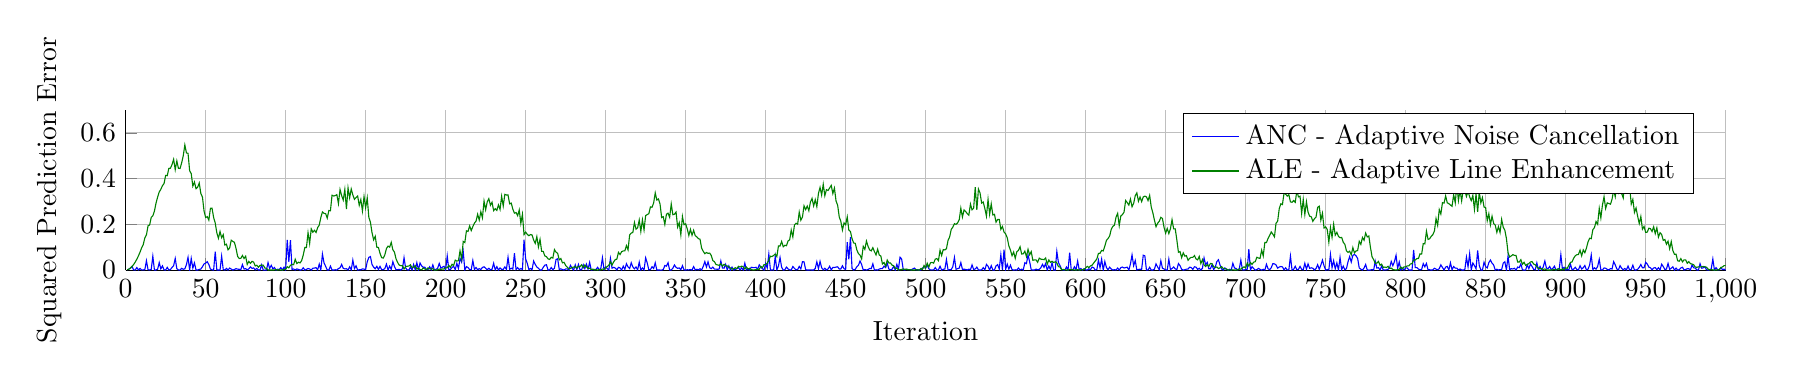
\begin{tikzpicture}

\begin{axis}[%
width=8in,
height=0.8in,
scale only axis,
xmin=0,
xmax=1000,
xlabel={Iteration},
xmajorgrids,
ymin=0,
ymax=0.7,
ylabel={Squared Prediction Error},
ymajorgrids,
axis x line*=bottom,
axis y line*=left,
legend style={draw=black,fill=white,legend cell align=left}
]
\addplot [color=blue,solid]
  table[row sep=crcr]{1	0.000986635785864219\\
2	0.00394264934276108\\
3	0.00885637463565566\\
4	0.0157084194356844\\
5	0.000729514535178227\\
6	0.000379728188170253\\
7	0.0109899608168079\\
8	0.00020894209396908\\
9	0.00686761239872795\\
10	0.000600551191384494\\
11	0.000969722875883411\\
12	0.00165050659308381\\
13	0.0410589534439609\\
14	0.00156113237744052\\
15	0.000472327222318902\\
16	0.00331019628956704\\
17	0.0605737905365236\\
18	0.000249473006948254\\
19	0.000460483097928274\\
20	0.00377965215009008\\
21	0.0328112382978347\\
22	0.00533286259928405\\
23	0.0182487769200106\\
24	0.000718676056659074\\
25	0.000223644685198702\\
26	0.0118036384984499\\
27	8.33530195385712e-06\\
28	0.00247016850769668\\
29	0.0114563159052859\\
30	0.0193201495253088\\
31	0.0507014983570395\\
32	0.0055854493489726\\
33	0.000750977304120338\\
34	1.28536000353463e-05\\
35	0.00756729459203954\\
36	0.00354060207393033\\
37	0.00527678603560538\\
38	0.023747540023016\\
39	0.0558265392771136\\
40	0.000509876182887205\\
41	0.051083802094015\\
42	0.00840523372918076\\
43	0.031384335524538\\
44	8.16394555084571e-05\\
45	0.000271086372617941\\
46	0.00282753975600059\\
47	0.00447668937433114\\
48	0.0145564016837587\\
49	0.0267932370996444\\
50	0.0305915952229966\\
51	0.0365414796894836\\
52	0.0242008075623838\\
53	0.00453166112442692\\
54	0.00109706743630847\\
55	2.25522708639825e-05\\
56	0.0803060132527195\\
57	0.000478535463867597\\
58	0.000139242466630674\\
59	5.86409561966463e-05\\
60	0.0607598646715718\\
61	0.00256089933634727\\
62	0.000380364000694818\\
63	0.00746653173212739\\
64	1.87980059112783e-05\\
65	0.00872888218704135\\
66	0.00432179229551607\\
67	0.000436894461391647\\
68	0.00238445643450923\\
69	0.00634563529973296\\
70	0.00401080412268283\\
71	0.00334565369338521\\
72	0.00237068597623857\\
73	0.0237456225230084\\
74	0.00446947192401238\\
75	0.00620007819476334\\
76	0.000182720923263631\\
77	0.00570212232268898\\
78	0.0137967896003303\\
79	0.00715266549942833\\
80	0.0095858631836582\\
81	0.000975770232128514\\
82	0.00719128907902827\\
83	0.000350054189544769\\
84	3.93108883210497e-05\\
85	0.0227055636075497\\
86	6.49967539303134e-07\\
87	8.92235974205668e-06\\
88	0.00030021470677156\\
89	0.032806991446316\\
90	0.00687293635634694\\
91	0.0209926449136966\\
92	0.00569404497403376\\
93	0.0110610547456582\\
94	1.59811974184444e-07\\
95	0.00373822218738657\\
96	0.00236808615181967\\
97	0.0105055503309835\\
98	0.000924525408623477\\
99	0.0124801880451173\\
100	6.02740596138542e-05\\
101	0.131733391706757\\
102	0.035687001379979\\
103	0.131261832115949\\
104	0.00285371493634501\\
105	0.00474789752012481\\
106	9.18167976620654e-05\\
107	0.00511648704888008\\
108	0.00291720609694084\\
109	5.33707265221011e-06\\
110	0.00110735337945239\\
111	0.0101195162828781\\
112	3.71327551241552e-06\\
113	0.00317160260985337\\
114	0.00666577967111714\\
115	0.00477833950600714\\
116	9.89996496390141e-05\\
117	0.00798329699707905\\
118	0.00863751726063609\\
119	0.0106090736841133\\
120	0.000846420270757568\\
121	0.0260019704291829\\
122	8.9702953760364e-05\\
123	0.0697568620467844\\
124	0.0315013833804035\\
125	0.0162647193802865\\
126	0.000215054682417464\\
127	0.000178608345222864\\
128	0.017414093280665\\
129	5.63450825670017e-10\\
130	0.000287401624062325\\
131	0.00137475887531528\\
132	1.69155737144458e-05\\
133	0.00648117739556179\\
134	0.010073313091184\\
135	0.0245940029174973\\
136	0.00772207394538773\\
137	0.00500693870864722\\
138	0.00591837455522933\\
139	0.000234905379653059\\
140	0.01442805823815\\
141	0.000711937530474572\\
142	0.043625588721068\\
143	0.00624261378909928\\
144	0.0185713523599876\\
145	0.00010130097792416\\
146	0.00144163958653651\\
147	0.00105420564695429\\
148	0.00526808015832193\\
149	0.00405508320468174\\
150	0.00240767407972845\\
151	0.036395151234124\\
152	0.0552948778454388\\
153	0.0589949318509731\\
154	0.0239044450590066\\
155	0.0127407909963272\\
156	0.0058176235420671\\
157	0.0162276097854063\\
158	0.00219666027220316\\
159	0.0160193871138103\\
160	0.00192296436057071\\
161	0.00206859219336738\\
162	0.00646594987991703\\
163	0.0259273770447387\\
164	2.25816357572163e-05\\
165	0.017027828425044\\
166	0.00322892290383221\\
167	0.0364610731473038\\
168	0.0154343321645782\\
169	0.00146059526343162\\
170	0.00206821796857836\\
171	0.00324533253895294\\
172	1.09307166325752e-06\\
173	0.00586589166854697\\
174	0.0542103986551576\\
175	0.00877540854775018\\
176	0.00092522653485592\\
177	1.2271898911318e-05\\
178	0.0134891003157671\\
179	3.05080347800373e-07\\
180	0.0248008557116898\\
181	0.00176070766718798\\
182	0.0322896094247333\\
183	0.00164887196464057\\
184	0.0308754721568498\\
185	0.0181791149887033\\
186	0.0122973826131574\\
187	0.0125782514536\\
188	0.00259570490456694\\
189	0.00229019812604363\\
190	0.0144796002506777\\
191	0.00199752029860768\\
192	0.0223380638526081\\
193	0.000340275269195722\\
194	0.00341078352578172\\
195	0.00772946248135471\\
196	0.0288867702275857\\
197	0.00863497770711801\\
198	0.0127653930945158\\
199	0.016410543440496\\
200	6.3501354201581e-06\\
201	0.0615905516366983\\
202	0.000989972974122228\\
203	0.00286804175856294\\
204	0.0111410963138039\\
205	0.0163660598655067\\
206	0.00189732625249749\\
207	0.0294004118804127\\
208	0.00692286842457009\\
209	0.0509567235530805\\
210	0.0345738905529036\\
211	0.0805739609606142\\
212	0.000280766564147394\\
213	0.0150482418721269\\
214	0.0110571567788922\\
215	0.00214408382233801\\
216	0.00157101220876567\\
217	0.0418675135841965\\
218	0.00279768145068956\\
219	0.0113986374574664\\
220	0.00137176138747305\\
221	0.00624296214288256\\
222	0.00265541276377635\\
223	0.0115166860428843\\
224	0.0142450952208844\\
225	0.00781572208283478\\
226	0.00162056941491719\\
227	0.00779786801564359\\
228	0.00114508999356133\\
229	0.00354506281764646\\
230	0.0295049222185939\\
231	0.00100254134931315\\
232	0.0151076380189582\\
233	1.83287779622789e-05\\
234	0.00946068269663368\\
235	0.00308976461297326\\
236	0.00309011796276625\\
237	0.0137325261098593\\
238	0.00324230342177405\\
239	0.0560720298228787\\
240	0.00306713623631833\\
241	0.00818358663442842\\
242	0.00417463804489611\\
243	0.073704926853575\\
244	0.00231020914168699\\
245	0.0106566507368182\\
246	0.00214640791585677\\
247	0.00657816340844587\\
248	0.00284069416961468\\
249	0.132497776086776\\
250	0.0487408068241763\\
251	0.0297249578029951\\
252	0.0023360935824541\\
253	0.00699724503666127\\
254	0.00145165079228841\\
255	0.039615273674808\\
256	0.0246893358041917\\
257	0.0134179789122548\\
258	0.00774370428920254\\
259	0.000194511399988469\\
260	4.6788909585161e-06\\
261	0.0118884995476618\\
262	0.0216417110901935\\
263	0.023428855292575\\
264	0.000114874444771468\\
265	0.000865959254116776\\
266	0.0111015980147741\\
267	0.00128400246724157\\
268	0.00772776255177874\\
269	0.0457232819817663\\
270	0.0498727281845507\\
271	0.00287154561211492\\
272	0.00546375518633629\\
273	0.002167600800866\\
274	0.000294128667111646\\
275	0.00463969433789491\\
276	0.00543493884483448\\
277	0.000148278087325787\\
278	0.0207012851418681\\
279	0.00813101780441993\\
280	4.38320126213507e-05\\
281	0.022620931439504\\
282	0.00172446886147962\\
283	0.0246436549770822\\
284	0.000941026601436788\\
285	0.00179938322123659\\
286	0.0230265286181813\\
287	0.00648424882890301\\
288	0.0260271961398583\\
289	0.00365002036890256\\
290	0.0337920402034536\\
291	0.000191041310724755\\
292	0.00127356648250768\\
293	0.0025849717169356\\
294	0.00268684774625981\\
295	0.0122802138858234\\
296	0.000788434159205033\\
297	0.00756872829902597\\
298	0.0537952369306467\\
299	0.00127206693559771\\
300	0.0135271715602919\\
301	0.0065334733831741\\
302	0.000167976713545235\\
303	0.0513143447070907\\
304	0.00844632622091292\\
305	0.0120461605164369\\
306	0.00885356039427447\\
307	0.000655502862008761\\
308	0.011965424472669\\
309	0.00934055146110165\\
310	0.000111193277495226\\
311	0.0170906063966022\\
312	0.00280349281061042\\
313	0.027819497700347\\
314	0.0140712802835382\\
315	0.00648441174280622\\
316	0.0318895916177978\\
317	0.0134969533844165\\
318	0.00544001788941915\\
319	0.0136574201876676\\
320	0.000719568962353424\\
321	0.0346682689650367\\
322	6.44657305455021e-07\\
323	0.00932740069483085\\
324	0.00031884600371829\\
325	0.0534407830044214\\
326	0.0309392244196038\\
327	0.000788802719247125\\
328	0.00230042641886238\\
329	0.0146360565644015\\
330	0.00675006613810618\\
331	0.0318856098662946\\
332	0.000106339242806798\\
333	0.000316906429034806\\
334	5.0908461817824e-05\\
335	1.52367930255803e-05\\
336	0.00203640623323573\\
337	0.0199677397523359\\
338	0.017231031412938\\
339	0.0322139211035987\\
340	5.22093743307887e-06\\
341	0.000377090893518266\\
342	0.00794955493674381\\
343	0.0224970748108859\\
344	0.0119022154577152\\
345	0.00742212652056484\\
346	0.00937426976958461\\
347	0.00166392114056951\\
348	0.0192726130732681\\
349	0.000785420322670543\\
350	6.81623120380828e-05\\
351	0.00138811174191555\\
352	0.000712648380033136\\
353	0.00224953298103728\\
354	0.000318644562549911\\
355	0.0153135190208433\\
356	0.000624725102179048\\
357	0.00331638333097847\\
358	0.00130351412867694\\
359	0.00578351803235462\\
360	0.000205198320431536\\
361	0.0162569042601824\\
362	0.0370599757460735\\
363	0.0133950393401688\\
364	0.0358882753447934\\
365	0.0102417184029388\\
366	0.00605959801241781\\
367	0.0126923964062066\\
368	0.00436779319716738\\
369	0.00429068048409198\\
370	0.00312638619920269\\
371	0.00514113138903155\\
372	0.039599637837449\\
373	0.00914048758237904\\
374	0.00820298167618298\\
375	0.0251664972692334\\
376	0.000704489638813784\\
377	0.0184304014661718\\
378	0.00013975804719107\\
379	0.0128607484913951\\
380	1.85372870542455e-05\\
381	0.00280045279512535\\
382	0.00560420313863336\\
383	0.0110883840398712\\
384	0.000407916204196643\\
385	0.00975372433821429\\
386	1.43865422230426e-06\\
387	0.0299692462194033\\
388	0.000430647378442132\\
389	0.00274039349685006\\
390	0.000359625197913611\\
391	0.0121878241678104\\
392	0.0109230524369447\\
393	0.0104778268091972\\
394	0.0122775631716728\\
395	0.00301812674872485\\
396	0.0229008853434592\\
397	0.0122634012525358\\
398	0.00585294605275243\\
399	0.000420538572191949\\
400	0.0284921828218406\\
401	0.00917880314420594\\
402	0.069830826149943\\
403	0.000332892901634499\\
404	0.000632581546890685\\
405	0.000479025951616164\\
406	0.0589951611467657\\
407	0.000417281426524022\\
408	0.0178653030508661\\
409	0.0545571140469943\\
410	0.0122609587170071\\
411	6.21138910183022e-05\\
412	0.00154521739628554\\
413	0.0130205467802026\\
414	0.00497732614829481\\
415	0.000989607098046299\\
416	0.000457705445709817\\
417	0.0155158537296922\\
418	0.00755401621190798\\
419	0.00126390309444349\\
420	0.00194255358142094\\
421	0.0157926459214855\\
422	0.00478052121659275\\
423	0.0362965470613439\\
424	0.0361022172355567\\
425	0.00181606196175132\\
426	9.67000308467483e-06\\
427	0.00026575075365982\\
428	0.000773146770310991\\
429	0.000322356207452488\\
430	2.82365581794669e-05\\
431	0.00669590570142445\\
432	0.0363639337484473\\
433	0.00603224831329984\\
434	0.0380624162352228\\
435	0.00995542902915246\\
436	0.00125974000454876\\
437	0.00797048887554739\\
438	0.000109820965084669\\
439	0.00484885365041278\\
440	0.0165474360685594\\
441	0.000646358939954427\\
442	0.0115879141553561\\
443	0.0113147045109264\\
444	0.0131807223283293\\
445	0.0142758671191137\\
446	0.00479636588761296\\
447	0.0047686449197008\\
448	0.018637671574516\\
449	0.00579561974070772\\
450	0.00242090934795825\\
451	0.121552967558552\\
452	0.0468258389754822\\
453	0.1435234111499\\
454	0.00700721838762728\\
455	0.000504131780158255\\
456	0.00323633638227985\\
457	0.0144618020847797\\
458	0.0210748807219808\\
459	0.039935584124588\\
460	0.0241846238529303\\
461	4.12887380620552e-05\\
462	0.002364038009188\\
463	0.000518259907637995\\
464	0.00205452954642123\\
465	0.00707324079586836\\
466	0.00608700807824884\\
467	0.0275594374213616\\
468	9.5394867226419e-05\\
469	0.0013335187544422\\
470	3.14461161264554e-05\\
471	0.00452404604201576\\
472	0.00619868920612412\\
473	0.00682023233461622\\
474	0.0174139539236179\\
475	0.0107600496364384\\
476	0.0299940111609206\\
477	0.00466267436320723\\
478	0.000295915668653107\\
479	0.00353085440260179\\
480	0.0163703943817108\\
481	0.000253854451520778\\
482	0.0248020541158328\\
483	0.00466446267371165\\
484	0.0563735628165175\\
485	0.0485329122531625\\
486	0.00221165281957025\\
487	1.80586719934734e-05\\
488	0.00330272740565776\\
489	0.00182211260189984\\
490	0.00221379228819355\\
491	0.000632494173168681\\
492	0.00542933149130478\\
493	0.00857038795723982\\
494	0.00115930250803022\\
495	0.00194707608890228\\
496	5.13491855829685e-06\\
497	0.000375938322177761\\
498	0.00896606561230546\\
499	0.00971615973842957\\
500	0.00905712097114889\\
501	0.0222345931444312\\
502	0.00573722224141089\\
503	0.000713410549062353\\
504	0.00075864654915655\\
505	0.000681421483383296\\
506	0.010875086934018\\
507	0.000169935404571441\\
508	0.000758282758680298\\
509	0.0167713372219816\\
510	0.000212261121121873\\
511	0.00352543666572614\\
512	0.0040576470806025\\
513	0.0457193613408975\\
514	0.000323711132466304\\
515	0.0019073982804403\\
516	0.00184911782910303\\
517	0.0150146629366553\\
518	0.0548136911065152\\
519	0.00352884619302812\\
520	0.00629814672828468\\
521	0.00851567079969795\\
522	0.0326518577731925\\
523	0.00289692096381443\\
524	0.00398094731772691\\
525	0.00282114318045801\\
526	0.000544876486179361\\
527	0.00410128950271728\\
528	0.00100926532142126\\
529	0.0225868532180658\\
530	0.00268839325814272\\
531	0.00497596152373432\\
532	0.0127789771395507\\
533	0.000619458570102773\\
534	1.16095501132134e-05\\
535	0.00107877418145735\\
536	0.0105657320505228\\
537	0.000815877472600555\\
538	0.0248546077545927\\
539	0.0167025609893722\\
540	7.17236088371887e-05\\
541	0.0191383518092395\\
542	0.000114274475198721\\
543	0.000189120075601216\\
544	0.0183471793229457\\
545	0.0237559896491543\\
546	0.00423497636279021\\
547	0.0673694695745572\\
548	0.000763092471154036\\
549	0.0894639247513431\\
550	0.00400629073149858\\
551	0.0258641917170746\\
552	0.0038638719413844\\
553	0.0213853737865275\\
554	0.00200004228801928\\
555	1.06086554187706e-05\\
556	0.00122718473701603\\
557	2.29089082165399e-05\\
558	0.00891090463956602\\
559	1.06908169352243e-05\\
560	0.00400938888690439\\
561	0.000313230582537303\\
562	0.0319114131188979\\
563	0.0281845875473346\\
564	0.0660657898230718\\
565	0.0364810847520196\\
566	0.000893777507459603\\
567	0.000445598453076211\\
568	0.000321385902387365\\
569	0.00418331499223371\\
570	0.00100800491123498\\
571	0.00338547169684524\\
572	0.0102105305071725\\
573	0.024961266117161\\
574	0.0117698064240344\\
575	0.0287019518190487\\
576	1.09774345063723e-05\\
577	0.0178693914603684\\
578	0.00157813725743386\\
579	0.0321697611800573\\
580	0.000367696079021371\\
581	4.62881386356028e-06\\
582	0.0817165503307811\\
583	0.0327290829894563\\
584	0.0194033212712315\\
585	0.00235406110160943\\
586	0.000435140493618462\\
587	0.000337385486851759\\
588	0.013316757171138\\
589	0.000107966610471383\\
590	0.0759801738651406\\
591	0.00155648755256557\\
592	0.000715672517697176\\
593	0.014555762394072\\
594	0.00154712401576494\\
595	0.0395795595290936\\
596	0.000216529106220381\\
597	0.00711447114991085\\
598	2.50189911286749e-06\\
599	0.00580059195531706\\
600	0.00105567043705866\\
601	8.49714267065601e-05\\
602	0.0052703977883294\\
603	0.0016065238771045\\
604	0.0131381124398228\\
605	0.0103652795403841\\
606	9.78274946825073e-05\\
607	0.00188308310918504\\
608	0.0433254802172225\\
609	0.0104676003219814\\
610	0.0478522881817983\\
611	2.60201846737472e-05\\
612	0.0373250047074869\\
613	0.0112486490213905\\
614	0.00105526640228756\\
615	0.0126183622393853\\
616	0.00457758365524677\\
617	0.00036521950545449\\
618	0.00174171394834321\\
619	0.000184621448126408\\
620	0.00892694732267117\\
621	0.000118043540763697\\
622	0.0106713717721301\\
623	0.0130931519907181\\
624	0.00904193317989257\\
625	0.0109012674634999\\
626	0.0126991693632699\\
627	2.76441883409682e-06\\
628	0.0267590144617413\\
629	0.0663478292818446\\
630	0.019247985118178\\
631	0.041674087197638\\
632	0.000390479378148825\\
633	0.00313598497828122\\
634	0.00344409417242926\\
635	0.00314732885083224\\
636	0.0649138677013271\\
637	0.062366519007874\\
638	0.000317772049079861\\
639	1.99306114651693e-05\\
640	0.0120692739474164\\
641	0.000173802311907634\\
642	3.98545701877076e-06\\
643	0.0040179048420867\\
644	0.0272240148167687\\
645	0.013284305863045\\
646	0.001507920694236\\
647	0.0406686357017913\\
648	0.00839468011026318\\
649	0.00470541303447872\\
650	0.00100502365067558\\
651	0.000186355885935945\\
652	0.047639098251417\\
653	0.00226226161356847\\
654	0.00680252093865736\\
655	0.0137191802129206\\
656	0.00523703510538321\\
657	0.00210533309407506\\
658	0.0283488880092724\\
659	0.0190943899202391\\
660	0.0037624053016154\\
661	3.30913268348502e-05\\
662	0.00140449308916554\\
663	0.00394299257910931\\
664	0.00454148969864663\\
665	0.0128025516505942\\
666	0.0107741715477384\\
667	0.00309109021637072\\
668	0.0143969147608228\\
669	0.0127916510811387\\
670	0.00292356316368553\\
671	0.00791169883741174\\
672	0.000456580165824237\\
673	0.00773009261827738\\
674	0.0529546783706616\\
675	0.0230962184393259\\
676	0.0332403536630812\\
677	0.005288218343582\\
678	0.00579254629896652\\
679	0.023489616076934\\
680	0.0022536977491485\\
681	0.0122618433958759\\
682	0.0374830369220011\\
683	0.044960991232008\\
684	0.0215689704978258\\
685	0.00440005634008233\\
686	2.94735409697763e-05\\
687	0.00955567723269218\\
688	0.0029591056974585\\
689	9.80502724451341e-05\\
690	0.00367367797345651\\
691	2.93299281274598e-06\\
692	0.0296181462727763\\
693	0.00895518738504266\\
694	0.00708934448722238\\
695	0.00088675544812127\\
696	0.0042002747488792\\
697	0.0437577976357116\\
698	0.000917029619175861\\
699	0.000431321133627866\\
700	0.00233868907696229\\
701	0.00400209577297333\\
702	0.0915182787802438\\
703	1.66915876844357e-05\\
704	0.0149046756066255\\
705	0.00678211064475911\\
706	0.000153331937809501\\
707	0.00168009857191424\\
708	0.00728118133497482\\
709	0.00292741199278934\\
710	1.2807341543878e-05\\
711	0.0033198531330952\\
712	9.73145283095821e-05\\
713	0.0254390861953975\\
714	0.00598829254494737\\
715	0.00132490980696107\\
716	0.0103382096809897\\
717	0.0277750081132776\\
718	0.0273251125275254\\
719	0.0226768294795925\\
720	0.00867366547258725\\
721	0.0132700807175523\\
722	0.0155362377412407\\
723	0.0138148707813399\\
724	0.00102460176741833\\
725	0.00983051349351784\\
726	0.000589558646778896\\
727	0.00103063776774568\\
728	0.0610775400358958\\
729	0.000143439090032756\\
730	0.00354797140377601\\
731	0.0166315390245637\\
732	0.00126623861567581\\
733	0.0033668667688578\\
734	0.016120517720573\\
735	0.00349832231099453\\
736	0.00123062702265858\\
737	0.0292220632426469\\
738	0.00378842235348451\\
739	0.0268395251098513\\
740	0.00766090270101726\\
741	0.00995242566347426\\
742	0.00782630451900599\\
743	0.000384807912291037\\
744	0.00676815818098599\\
745	0.023394369406428\\
746	0.00323405667032982\\
747	0.0213603205280077\\
748	0.0435368140400369\\
749	0.0190440611372175\\
750	2.04589388315688e-05\\
751	0.00225102149365964\\
752	0.000304183820360789\\
753	0.0684319016745767\\
754	0.0104886502297625\\
755	0.0411064102596788\\
756	0.00556842040628616\\
757	0.0310884249749316\\
758	0.000142005707662661\\
759	0.05536617669786\\
760	0.00162819331072528\\
761	0.017314760989655\\
762	0.00138805020860988\\
763	0.00638705418657309\\
764	0.0367797637591326\\
765	0.0589107250165034\\
766	0.0350058695290751\\
767	0.0641243907501934\\
768	0.0682002545094163\\
769	0.0624542182057675\\
770	0.0506829908881975\\
771	0.0094705883990432\\
772	0.00365615015179517\\
773	7.63889482793135e-05\\
774	0.00886104599102661\\
775	0.0244646840321587\\
776	0.000191362371221594\\
777	9.60612455711298e-06\\
778	0.000118128594748989\\
779	0.00225935260324634\\
780	6.54568560993244e-06\\
781	0.0389158432039046\\
782	0.00867222407974468\\
783	0.0105951828595946\\
784	1.38337937764209e-06\\
785	0.0176288971305534\\
786	0.000153457685987922\\
787	0.000870851094757496\\
788	0.000664776226329917\\
789	0.00321138051892911\\
790	0.0100879803505394\\
791	0.0375932371727653\\
792	0.018932374593285\\
793	0.036597984441632\\
794	0.064466934232087\\
795	0.00756673880089274\\
796	0.0352335584478803\\
797	0.000179736032871431\\
798	0.00799388850091499\\
799	6.14010351466375e-08\\
800	0.00914629817036486\\
801	0.00969263382600882\\
802	0.000306731867661734\\
803	8.71880146273518e-05\\
804	0.000254641591467723\\
805	0.0877039564871253\\
806	0.0111915932502982\\
807	0.0107225790652214\\
808	0.0046432270793032\\
809	0.000987794633332646\\
810	0.00273219534421358\\
811	0.0282363250176912\\
812	0.0142007439672201\\
813	0.0288326426422953\\
814	0.00100527807461947\\
815	0.00134399873729724\\
816	0.000134663569999304\\
817	0.000864375518169786\\
818	0.00809539162546519\\
819	0.00396366887931631\\
820	0.000997143877240424\\
821	0.00610120231993246\\
822	0.0227990554042657\\
823	0.0115442286803835\\
824	4.24772359328467e-05\\
825	0.0130068430435562\\
826	0.0159791155853661\\
827	0.0001846772965999\\
828	0.0314716469639623\\
829	0.00167292341415966\\
830	0.0150139611777735\\
831	0.00819580947291384\\
832	0.00854411245000551\\
833	6.9173915703664e-05\\
834	0.00477682242842038\\
835	0.000339196895351961\\
836	0.00011857485118625\\
837	0.00261747217960127\\
838	0.0566493427074209\\
839	0.0146256462295633\\
840	0.0715042340029285\\
841	0.000548521899501108\\
842	0.0308843841465202\\
843	0.0192612395647512\\
844	0.00559400509562478\\
845	0.085655718280434\\
846	0.0208151727495274\\
847	0.00033259041382809\\
848	0.000167019339691167\\
849	0.0341534478558347\\
850	0.015020750775946\\
851	0.00930144592088664\\
852	0.0326594988360758\\
853	0.0437767355467756\\
854	0.0302503550557452\\
855	0.022354933094646\\
856	9.17316863219455e-06\\
857	0.00382918283721117\\
858	4.94232589159303e-05\\
859	0.00220140029218595\\
860	0.00225412999583735\\
861	0.0304407211666868\\
862	0.0363294923792297\\
863	1.74810447240992e-05\\
864	0.0620822522883619\\
865	0.000764745902330782\\
866	0.00641253947837549\\
867	0.00486018672010595\\
868	0.00794249515144536\\
869	1.76308905255564e-05\\
870	0.0132223034427688\\
871	0.0107704131205303\\
872	0.0272957541845668\\
873	0.000965373574613218\\
874	6.66638537468488e-05\\
875	1.47369008473004e-05\\
876	0.0230680925365186\\
877	0.00593904841418603\\
878	0.0265534693724641\\
879	0.0160441761605858\\
880	0.00290336808642503\\
881	0.00114899516953875\\
882	0.0313606390814311\\
883	3.0014707946659e-05\\
884	0.0156088304081709\\
885	0.000601927662776389\\
886	0.0142940595959616\\
887	0.0395584866720272\\
888	0.00861739874480806\\
889	0.00626284350878716\\
890	0.0154424998643709\\
891	0.00143263866630876\\
892	0.00741401679111066\\
893	0.0168219350970227\\
894	1.53131463097473e-05\\
895	0.00523892798432569\\
896	0.00376414159616538\\
897	0.0675114010006458\\
898	0.00355818343884158\\
899	0.0120297410501148\\
900	0.000598237591279946\\
901	0.00195796879662297\\
902	0.000624932949086467\\
903	0.025939884116466\\
904	0.00162776021874333\\
905	0.00401411911108671\\
906	0.0121914031095413\\
907	0.00275062095927381\\
908	0.000619625743240612\\
909	0.0190938809552083\\
910	0.00453508786886948\\
911	0.0100965481566106\\
912	0.0198281022071716\\
913	0.000439089754245112\\
914	0.00425955655179598\\
915	0.0223674145129951\\
916	0.0658031825756466\\
917	0.00215060911441896\\
918	0.00995603360377534\\
919	0.00394462286720894\\
920	0.0158674649496844\\
921	0.0469591583099312\\
922	0.000636300333445008\\
923	0.000532277674646157\\
924	0.00913338136783065\\
925	0.00821137200121348\\
926	0.00290457054228339\\
927	0.000486523811620788\\
928	0.0063912045540998\\
929	0.00471339073718448\\
930	0.0367005595970567\\
931	0.022705992983332\\
932	0.00454606182720926\\
933	0.00112427812506402\\
934	0.0192171261845253\\
935	0.00827492566059097\\
936	0.000944619631519795\\
937	0.00705472672280629\\
938	0.000926053185064946\\
939	0.0176120341555844\\
940	0.000203616876859881\\
941	0.00277109257782551\\
942	0.0214751146808646\\
943	0.000718906451676297\\
944	2.10714274858875e-05\\
945	0.00345338129628413\\
946	0.0119371820900534\\
947	0.0245303360859646\\
948	0.0100202452034475\\
949	0.0103219820630052\\
950	0.033860644359073\\
951	0.0264040900895748\\
952	0.013051930412826\\
953	0.0100295409284315\\
954	0.00126884702944145\\
955	0.00919363433468118\\
956	0.0108312081385731\\
957	0.00175207790059056\\
958	0.0101660790199204\\
959	0.00025891933412383\\
960	0.025811212427032\\
961	0.0154144168595318\\
962	0.00241427182892136\\
963	0.00447331964261702\\
964	0.0291125277927648\\
965	0.00284597408024866\\
966	0.00805512384004264\\
967	0.0140696423358307\\
968	0.000150935634369381\\
969	0.00860252444788297\\
970	0.000104362963267495\\
971	0.00163840383196527\\
972	0.00940243307223326\\
973	0.0124182208723445\\
974	0.000608772330360862\\
975	0.00246631099421224\\
976	0.00580879800249355\\
977	0.00580100815940511\\
978	0.000802043292479919\\
979	0.0223414666084734\\
980	0.00991071576883658\\
981	0.00884052743223541\\
982	0.000386893555177762\\
983	0.000285917140177459\\
984	0.0279082096739422\\
985	0.00818219722426608\\
986	0.00982824253487619\\
987	0.0150206802665234\\
988	0.00150868425322528\\
989	0.000309720939277404\\
990	0.000749998885478375\\
991	0.00565526659742761\\
992	0.0485079237796039\\
993	2.54487762766989e-05\\
994	0.010518189772968\\
995	0.00120575758485613\\
996	0.000652261086901245\\
997	0.0106170958437245\\
998	0.00211571246215377\\
999	0.00417521623847857\\
1000	0.000110984546085945\\
};
\addlegendentry{ANC - Adaptive Noise Cancellation};

\addplot [color=black!50!green,solid]
  table[row sep=crcr]{1	0.000986635785864219\\
2	0.00394264934276108\\
3	0.00885637463565566\\
4	0.0157084194356844\\
5	0.0244717418524232\\
6	0.0351117570558743\\
7	0.0475864737669902\\
8	0.0621976105274847\\
9	0.0785110892583809\\
10	0.097285646555178\\
11	0.111365081726094\\
12	0.140614465435779\\
13	0.153969645861913\\
14	0.193447154085585\\
15	0.197173312601885\\
16	0.230443810471058\\
17	0.237454188307969\\
18	0.258221561941443\\
19	0.292880405726426\\
20	0.31954422083789\\
21	0.341834663803863\\
22	0.353087817731293\\
23	0.369171417932605\\
24	0.378354063716672\\
25	0.413889070933113\\
26	0.412816914467822\\
27	0.444902615502394\\
28	0.445596540376301\\
29	0.461684265098447\\
30	0.484567369245486\\
31	0.439197945211713\\
32	0.477483605552868\\
33	0.444958703620885\\
34	0.444459528973612\\
35	0.468497161175447\\
36	0.499591936860219\\
37	0.547213696648174\\
38	0.512325173549179\\
39	0.510812857014317\\
40	0.434534821413661\\
41	0.42177129741454\\
42	0.367248664734618\\
43	0.385151138289168\\
44	0.355961831042523\\
45	0.362399533952095\\
46	0.380957779073526\\
47	0.335211458339791\\
48	0.319580839622299\\
49	0.258633735131807\\
50	0.229970309760355\\
51	0.233789875763051\\
52	0.218440057930633\\
53	0.270211125465944\\
54	0.270706274848183\\
55	0.229717636298047\\
56	0.20578449444036\\
57	0.162667599581738\\
58	0.139340828869804\\
59	0.168735893472595\\
60	0.141412494682818\\
61	0.155288428113488\\
62	0.109653709673234\\
63	0.113268876127346\\
64	0.0884819982932122\\
65	0.0964397692214556\\
66	0.130667295977035\\
67	0.125354540976594\\
68	0.121400314283967\\
69	0.0943157576602905\\
70	0.0598931111813358\\
71	0.0506853249814236\\
72	0.0513164186203643\\
73	0.0637736938971613\\
74	0.0504779235224667\\
75	0.0606392338470935\\
76	0.0246793399145585\\
77	0.03771949397402\\
78	0.0293659942521939\\
79	0.0381383031168256\\
80	0.0346196979034696\\
81	0.0181174315300816\\
82	0.0210981600884475\\
83	0.0121541943978144\\
84	0.0207553393088314\\
85	0.0212820304056431\\
86	0.0215752328715048\\
87	0.00916577416803881\\
88	0.00743710056408518\\
89	0.000445501657912949\\
90	0.000556570162940901\\
91	0.000179479867332203\\
92	3.0807873597671e-05\\
93	0.000637069981674024\\
94	0.00231703632599192\\
95	1.77837030415919e-07\\
96	0.00188334818459347\\
97	1.5764283209172e-05\\
98	0.000118812987827369\\
99	0.00235057609813473\\
100	0.00275437855456591\\
101	0.0147364136910464\\
102	0.00980166459884725\\
103	0.0210009592901748\\
104	0.0241288662107337\\
105	0.0234981803719517\\
106	0.0472480003006903\\
107	0.0284706646291661\\
108	0.0343887009581874\\
109	0.0313534179144044\\
110	0.0411842839929398\\
111	0.0656880701551844\\
112	0.0985972437609722\\
113	0.0987785185709757\\
114	0.163631802017426\\
115	0.116110409854239\\
116	0.180471982562233\\
117	0.165564964596084\\
118	0.173887203518601\\
119	0.164587405548095\\
120	0.185753605202631\\
121	0.196587639763436\\
122	0.229846133887281\\
123	0.254254840457538\\
124	0.248337361627449\\
125	0.246683706678832\\
126	0.227128242845868\\
127	0.260414565502635\\
128	0.259613985355069\\
129	0.327618049826209\\
130	0.323901868490968\\
131	0.325748327185434\\
132	0.329945620205672\\
133	0.29079925757665\\
134	0.352544162817135\\
135	0.325972149308304\\
136	0.306219387011495\\
137	0.352908923343923\\
138	0.266888150639653\\
139	0.35963229057624\\
140	0.31598111081377\\
141	0.354935205371353\\
142	0.328861318278956\\
143	0.309576447461736\\
144	0.317410269673402\\
145	0.324132170547463\\
146	0.283270363374369\\
147	0.308549560499087\\
148	0.258850192331725\\
149	0.321381022226171\\
150	0.272432570122376\\
151	0.315970591425849\\
152	0.230767482518782\\
153	0.208866321453682\\
154	0.163207357395175\\
155	0.132313384691206\\
156	0.147618019520305\\
157	0.099939831403278\\
158	0.098590467253507\\
159	0.0728826583503303\\
160	0.0544303741230594\\
161	0.0523805572870973\\
162	0.06667356547777\\
163	0.093968622210506\\
164	0.104725333459874\\
165	0.100377673867685\\
166	0.121339611017733\\
167	0.0890144412602912\\
168	0.0786029928334842\\
169	0.0490245137511252\\
170	0.0330376906879935\\
171	0.0216874472587634\\
172	0.019260306127004\\
173	0.0187855522280145\\
174	0.00457249237101024\\
175	0.0152759728752517\\
176	0.0167308832654927\\
177	0.0174872749014788\\
178	0.023379656547346\\
179	0.0101414852600982\\
180	0.013000000467937\\
181	0.0194854703582289\\
182	0.00403225396863339\\
183	0.00829735937441321\\
184	0.00241529503207184\\
185	0.00166349161494964\\
186	0.00904958716433211\\
187	0.00449871549173602\\
188	0.00154023953201649\\
189	0.00934438614935861\\
190	0.00504461877964051\\
191	0.00477786720836306\\
192	0.00581277903305413\\
193	1.88334642358263e-07\\
194	5.349260669387e-05\\
195	0.0011947261165727\\
196	0.00440802561101893\\
197	0.0026901832652512\\
198	0.00493960214638122\\
199	0.00454347600891214\\
200	0.00951494416400944\\
201	0.0101224068269769\\
202	0.020222110133278\\
203	0.0121003909512664\\
204	0.0254589649645673\\
205	0.0199626131719468\\
206	0.0435576785790099\\
207	0.0391150319170799\\
208	0.0413339160575334\\
209	0.0842579754008538\\
210	0.048767603951174\\
211	0.125187834596746\\
212	0.120417547628997\\
213	0.171567650279445\\
214	0.169316742916028\\
215	0.193117683468997\\
216	0.172542887571643\\
217	0.19019128260289\\
218	0.205465954861231\\
219	0.213990113975915\\
220	0.244245292604382\\
221	0.218716607061261\\
222	0.254942335781889\\
223	0.228999474168111\\
224	0.301911925950961\\
225	0.263657317977099\\
226	0.298236518630536\\
227	0.312197993202901\\
228	0.2836834446349\\
229	0.296728935312755\\
230	0.259954075357422\\
231	0.26852398341564\\
232	0.26094631843948\\
233	0.285110151474511\\
234	0.264901536210808\\
235	0.322632632111151\\
236	0.280244203822798\\
237	0.331232466237045\\
238	0.328347962601959\\
239	0.328300351970687\\
240	0.28987007478262\\
241	0.293119684292162\\
242	0.26637069812579\\
243	0.249101811998812\\
244	0.251576063692717\\
245	0.237554762282054\\
246	0.263065010298103\\
247	0.204187778825918\\
248	0.243801498465093\\
249	0.155187801173748\\
250	0.166169799370451\\
251	0.156504235784576\\
252	0.150056205070327\\
253	0.155376546850123\\
254	0.153631667917669\\
255	0.131532577375023\\
256	0.116714912630229\\
257	0.146257443331882\\
258	0.100858859778208\\
259	0.134341675211099\\
260	0.0821006369216727\\
261	0.0813873841523546\\
262	0.0617535651370058\\
263	0.0588582821006468\\
264	0.048804197662933\\
265	0.0465106769383504\\
266	0.0559010037205736\\
267	0.0525621914597438\\
268	0.0895175560966536\\
269	0.078096211263876\\
270	0.073548168742754\\
271	0.0448543897891684\\
272	0.0506594178348397\\
273	0.0317047987696459\\
274	0.0338409615754363\\
275	0.0201810628971443\\
276	0.0126633230390553\\
277	0.00528379782401281\\
278	0.00741578682433157\\
279	0.0113160580030776\\
280	0.0129328401160382\\
281	0.0157725239194252\\
282	0.00812298658105081\\
283	0.0163441422229899\\
284	0.0149513884914361\\
285	0.0232635343646576\\
286	0.0104835316831447\\
287	0.0217537657365749\\
288	0.0146354806764041\\
289	0.0081085201098345\\
290	0.00820025497776929\\
291	0.00220907209272508\\
292	0.00413290102271773\\
293	0.00048245606278418\\
294	0.0015986410243086\\
295	1.60881232398334e-05\\
296	0.00198961600683355\\
297	0.00128810432194344\\
298	0.00446609436283809\\
299	0.00336970319340742\\
300	0.00983330596233827\\
301	0.0153710468977748\\
302	0.0214818494782165\\
303	0.0364506948506063\\
304	0.0214601712826312\\
305	0.0356273354808283\\
306	0.0459880537908485\\
307	0.0476066776983004\\
308	0.0775256973004159\\
309	0.0679934956705932\\
310	0.0804846926193735\\
311	0.0836614642447593\\
312	0.0840866841648743\\
313	0.107120022123573\\
314	0.0883408299249856\\
315	0.153823897105708\\
316	0.161849358142042\\
317	0.164408215690455\\
318	0.207950353884872\\
319	0.179023634005722\\
320	0.185143178589281\\
321	0.219059836948621\\
322	0.168862305157211\\
323	0.220222316756728\\
324	0.175772953602791\\
325	0.23826159676581\\
326	0.242995502916066\\
327	0.246614438420181\\
328	0.276349614835266\\
329	0.274717486407945\\
330	0.293666415623655\\
331	0.337683123930777\\
332	0.30623444126687\\
333	0.310861331274919\\
334	0.28916012747385\\
335	0.229727474370915\\
336	0.233720379844635\\
337	0.199619404382761\\
338	0.24401516004442\\
339	0.24911896277325\\
340	0.230917735408122\\
341	0.289053878701925\\
342	0.242282759238721\\
343	0.24418235208269\\
344	0.253844999116235\\
345	0.187772032937301\\
346	0.207163748056158\\
347	0.154067316412481\\
348	0.234148622926016\\
349	0.198611977638145\\
350	0.202316700936835\\
351	0.180341757143217\\
352	0.15108142571718\\
353	0.178168212299071\\
354	0.152037701715485\\
355	0.173858517724967\\
356	0.150572323417277\\
357	0.1453122131442\\
358	0.137177825548614\\
359	0.135012963207709\\
360	0.0955845662632088\\
361	0.0823843350516011\\
362	0.0715754035650924\\
363	0.0768253651069486\\
364	0.0732825734509896\\
365	0.0742972469867533\\
366	0.0638308322264497\\
367	0.0414286825337932\\
368	0.0365882637303648\\
369	0.0242425439324528\\
370	0.0223857667316745\\
371	0.0208210380911913\\
372	0.0278774981832889\\
373	0.0170062607364258\\
374	0.0252120943079441\\
375	0.0192812376371155\\
376	0.0179439342038444\\
377	0.013393913661719\\
378	0.00894193861211083\\
379	0.00405566947934867\\
380	0.00504616327062533\\
381	0.0102298681685147\\
382	0.00607094653274277\\
383	0.0164783556352646\\
384	0.0134446977762131\\
385	0.0172120149350514\\
386	0.0142519815015635\\
387	0.00478186186695455\\
388	0.0133591488983074\\
389	0.00445996263761729\\
390	0.00787308700906401\\
391	0.00244033825593731\\
392	0.000586271588946293\\
393	0.000840524719124938\\
394	0.00255596149488873\\
395	0.00364733869226684\\
396	0.0029602920122294\\
397	0.0160596116549444\\
398	0.0110885933020219\\
399	0.0236685934465376\\
400	0.0237919911391103\\
401	0.0302732888041548\\
402	0.0432327321031861\\
403	0.0605232518589322\\
404	0.0590987557642095\\
405	0.0639194394179875\\
406	0.0701451329862187\\
407	0.058764290722357\\
408	0.105288934727494\\
409	0.105248231865905\\
410	0.12521199661543\\
411	0.102065157883862\\
412	0.108557619572514\\
413	0.106494719434656\\
414	0.127313199286503\\
415	0.132186166709608\\
416	0.175076812362157\\
417	0.144948762105311\\
418	0.197044022456803\\
419	0.204913937156355\\
420	0.20071151724121\\
421	0.253601962462837\\
422	0.217730851956041\\
423	0.231768766340281\\
424	0.28099790522534\\
425	0.264375312547865\\
426	0.279901597957991\\
427	0.259744114989193\\
428	0.297829050656135\\
429	0.313522137392945\\
430	0.280719824963198\\
431	0.308028590284598\\
432	0.277457482727827\\
433	0.334635101790333\\
434	0.361672190806965\\
435	0.328359992120675\\
436	0.375600222793028\\
437	0.325109023318531\\
438	0.351936489094324\\
439	0.348184123608212\\
440	0.359115787093879\\
441	0.370634507439355\\
442	0.334647367674036\\
443	0.358658662589975\\
444	0.301908982270992\\
445	0.283819698721207\\
446	0.232676164361553\\
447	0.212940516868533\\
448	0.17503862122361\\
449	0.206496190281677\\
450	0.198319915676303\\
451	0.232632008332984\\
452	0.174875716487422\\
453	0.168588859874233\\
454	0.137452415306409\\
455	0.118674974078205\\
456	0.117046151746325\\
457	0.0880678665050772\\
458	0.0719318995260951\\
459	0.065280852717926\\
460	0.0487937393195095\\
461	0.103636785293043\\
462	0.0908137749303769\\
463	0.126860252736927\\
464	0.103962996520618\\
465	0.0883380685867863\\
466	0.0839385991366823\\
467	0.0977989197614167\\
468	0.0806464463993086\\
469	0.0665024293087344\\
470	0.0912394648894453\\
471	0.066006876157541\\
472	0.0615607440428154\\
473	0.026592460462205\\
474	0.0331614192289429\\
475	0.0169230311329158\\
476	0.0438652805874814\\
477	0.0310872276935794\\
478	0.0310817148617603\\
479	0.0214968710375394\\
480	0.0193011796141105\\
481	0.00716024809535733\\
482	0.00864717058230428\\
483	0.000784083104595225\\
484	0.00140235163773801\\
485	0.00256401229180701\\
486	0.00508695593907014\\
487	0.00321843972286578\\
488	0.00389507300448838\\
489	0.00212983326331901\\
490	0.0021557141758912\\
491	7.42223404751623e-05\\
492	0.000404791462351152\\
493	0.000302363909149055\\
494	0.00165737495482535\\
495	0.000412955749691291\\
496	4.7626027992741e-05\\
497	0.00695855495913776\\
498	0.002843538388761\\
499	0.0200558705809067\\
500	0.00877129472181547\\
501	0.029908104934398\\
502	0.0132689373948905\\
503	0.0318115013816668\\
504	0.0334448370082848\\
505	0.0303247677580661\\
506	0.0477680336311741\\
507	0.0502217284872425\\
508	0.0412761194395837\\
509	0.0869716094955494\\
510	0.0637435167196738\\
511	0.0896148105889481\\
512	0.0879956116944332\\
513	0.0934196748376671\\
514	0.129756985083677\\
515	0.14507046082074\\
516	0.177718175311078\\
517	0.187966441843653\\
518	0.203074351365479\\
519	0.199940864868813\\
520	0.206405999474869\\
521	0.220345318326905\\
522	0.270842028281373\\
523	0.232076990415971\\
524	0.26299793388123\\
525	0.256413293820017\\
526	0.246905918883503\\
527	0.240263506141981\\
528	0.288643874627939\\
529	0.263393942592399\\
530	0.270670392534339\\
531	0.36300970069208\\
532	0.263458287354206\\
533	0.354726298041496\\
534	0.337251002103816\\
535	0.293238967222997\\
536	0.297707278828045\\
537	0.269356508802486\\
538	0.235922620544494\\
539	0.30902983873795\\
540	0.244117413746988\\
541	0.289438759685379\\
542	0.241028087905921\\
543	0.244017567300883\\
544	0.20960701851275\\
545	0.221237645781089\\
546	0.2217328150618\\
547	0.178135466087143\\
548	0.190653649759812\\
549	0.166144049712802\\
550	0.158298522506068\\
551	0.141337083740698\\
552	0.10592926305177\\
553	0.0874634872413041\\
554	0.0628867592456435\\
555	0.0790311108517072\\
556	0.0515581567146323\\
557	0.0804307271877543\\
558	0.0859481889800724\\
559	0.102140596470095\\
560	0.0704310189330867\\
561	0.0706107799300788\\
562	0.0827719392670246\\
563	0.0589592086762897\\
564	0.0906651303651111\\
565	0.0666903577387133\\
566	0.08039957327308\\
567	0.0427100514751337\\
568	0.0443012601212398\\
569	0.0445458817407279\\
570	0.0342441665255342\\
571	0.052150237540912\\
572	0.0475777183393578\\
573	0.0468894757939247\\
574	0.045434939935341\\
575	0.0531118087572005\\
576	0.0256860594543062\\
577	0.0441244795222945\\
578	0.0336615509652884\\
579	0.0378652957172002\\
580	0.0329944121862795\\
581	0.0363108409845067\\
582	0.0309427630796928\\
583	0.0150619599939443\\
584	0.013124398146595\\
585	0.00117652524734517\\
586	0.00282160671171804\\
587	0.00108614644422377\\
588	0.000733514832659901\\
589	1.13756118267969e-05\\
590	0.00309334550293104\\
591	0.0019512801286619\\
592	0.00111816333710408\\
593	0.000879575732390462\\
594	0.000122866212024927\\
595	0.0021438649966739\\
596	7.41505540145498e-05\\
597	0.000603260085719648\\
598	0.00171497027374291\\
599	0.00278257909676244\\
600	0.00912281857937444\\
601	0.0164552080350541\\
602	0.0105944122851406\\
603	0.0180779526412519\\
604	0.0210697114176552\\
605	0.0305784663587572\\
606	0.039672922821017\\
607	0.0483161423634071\\
608	0.0728859225424194\\
609	0.0736763427118014\\
610	0.0860018799575017\\
611	0.083582370254966\\
612	0.105096421688244\\
613	0.129876423948525\\
614	0.138132857306565\\
615	0.14909215850346\\
616	0.178150614478536\\
617	0.191213343660004\\
618	0.196305000645236\\
619	0.231521770735861\\
620	0.24808273281535\\
621	0.194453020508955\\
622	0.237429023359481\\
623	0.242602567141137\\
624	0.253661554768328\\
625	0.304272498945163\\
626	0.295181516387579\\
627	0.284184246088319\\
628	0.310836524264143\\
629	0.27712241364855\\
630	0.291741590019186\\
631	0.325237476554735\\
632	0.337697770120386\\
633	0.301085696539323\\
634	0.319712636622217\\
635	0.299286107728486\\
636	0.319737608811419\\
637	0.323359946539192\\
638	0.320358880188965\\
639	0.304094740464125\\
640	0.326858684673194\\
641	0.276191381313438\\
642	0.250522443354174\\
643	0.218107662310176\\
644	0.189710902369001\\
645	0.205021220389211\\
646	0.213206354696845\\
647	0.230670471566659\\
648	0.225618028965536\\
649	0.186993065463514\\
650	0.161473116545197\\
651	0.181847341013721\\
652	0.159622529603401\\
653	0.180953694007029\\
654	0.220631629468196\\
655	0.180097485715479\\
656	0.180336781364897\\
657	0.131695479944279\\
658	0.0778710576966549\\
659	0.0807920036724952\\
660	0.0540075608668252\\
661	0.075240641696231\\
662	0.0607472721123742\\
663	0.0630113413928494\\
664	0.042643006971417\\
665	0.0513498684066151\\
666	0.0556635476429356\\
667	0.0555747046299724\\
668	0.0633140314816674\\
669	0.0488216430020926\\
670	0.0444324899039543\\
671	0.059724579608797\\
672	0.0281876414033614\\
673	0.0455679669894142\\
674	0.0224254735588283\\
675	0.0153021950318368\\
676	0.0234529217538513\\
677	0.0157918644071023\\
678	0.0291716321355729\\
679	0.0280319693222683\\
680	0.0151181977007927\\
681	0.011511413979888\\
682	0.0133509775675155\\
683	0.0064332586948449\\
684	0.00994113453639042\\
685	0.0153224830314609\\
686	0.00642947889271896\\
687	0.00514765223243245\\
688	0.00514400987026026\\
689	7.4229785114194e-06\\
690	0.00082378679309473\\
691	7.36139586272854e-05\\
692	0.00118327262541439\\
693	0.000332002340870019\\
694	6.42163073492841e-05\\
695	0.000603410109379004\\
696	0.00508211770356925\\
697	0.00369225737501409\\
698	0.0097610882304464\\
699	0.014161280926214\\
700	0.00967447546961319\\
701	0.0301592050247081\\
702	0.0174301776845055\\
703	0.0330711446700272\\
704	0.0248187515638972\\
705	0.0345104580302757\\
706	0.0366490882911751\\
707	0.055975496129256\\
708	0.05269155061373\\
709	0.0509903248595901\\
710	0.0873013163888102\\
711	0.0618679013455789\\
712	0.120901197904524\\
713	0.120052366118184\\
714	0.13827680247418\\
715	0.151584055748852\\
716	0.166636752017689\\
717	0.157122143824035\\
718	0.145315121865129\\
719	0.205056624126601\\
720	0.213613457134995\\
721	0.268264419633791\\
722	0.290012669469348\\
723	0.286777609148567\\
724	0.336985196327679\\
725	0.332180145516258\\
726	0.323784739339363\\
727	0.32974878999814\\
728	0.298500447462188\\
729	0.296414868523699\\
730	0.304238905739803\\
731	0.296223234755119\\
732	0.347355815868712\\
733	0.32019785184347\\
734	0.323021394338054\\
735	0.247919097155948\\
736	0.308983073218636\\
737	0.24341323711508\\
738	0.299028285214395\\
739	0.253607845152785\\
740	0.235867097503219\\
741	0.233243456553882\\
742	0.213180829473742\\
743	0.224775232935973\\
744	0.232224753164026\\
745	0.274297691027519\\
746	0.279441520316404\\
747	0.218447758298445\\
748	0.248754517790671\\
749	0.183786503594151\\
750	0.189003368111979\\
751	0.177220664325596\\
752	0.121731556552644\\
753	0.186003298290938\\
754	0.143514521379993\\
755	0.200819047134981\\
756	0.152782839758579\\
757	0.165146241506101\\
758	0.147541801450135\\
759	0.141417367230182\\
760	0.142762325626254\\
761	0.121699635491536\\
762	0.1127417811752\\
763	0.0843295811574707\\
764	0.0775653587739386\\
765	0.08255608863724\\
766	0.0664545553681377\\
767	0.098250298676249\\
768	0.0749679388965015\\
769	0.0837991360996089\\
770	0.0851307101372867\\
771	0.125916381762338\\
772	0.11231617598196\\
773	0.142577465141654\\
774	0.130484134483121\\
775	0.161786892775715\\
776	0.144877672798372\\
777	0.148877394202766\\
778	0.0994575000417183\\
779	0.0578917983582788\\
780	0.0456735180498409\\
781	0.029689253498269\\
782	0.0302997003724683\\
783	0.0378596018002823\\
784	0.0212202194035933\\
785	0.0261730748570289\\
786	0.0112397941715211\\
787	0.013144084798608\\
788	0.0112305079367811\\
789	0.0164748285344572\\
790	0.00696056525116335\\
791	0.00866655760864155\\
792	0.00231166246561751\\
793	0.00109316751440826\\
794	0.00011289928618286\\
795	0.00175366133058101\\
796	0.00340780482435949\\
797	0.0130982560824745\\
798	0.00554811269383267\\
799	0.0141664991745169\\
800	0.0137287833433361\\
801	0.0181107964952961\\
802	0.0181946117781\\
803	0.02688881101608\\
804	0.0279097028811122\\
805	0.0448191898695076\\
806	0.0434327981346791\\
807	0.0502444539113077\\
808	0.0508457799903142\\
809	0.0710280931944822\\
810	0.0699097512276958\\
811	0.11572887615742\\
812	0.114575384324172\\
813	0.170099584546314\\
814	0.13416588922753\\
815	0.136865785164364\\
816	0.147715901246158\\
817	0.154959762719625\\
818	0.171111667755882\\
819	0.22539456067982\\
820	0.19585773516489\\
821	0.264393812304991\\
822	0.245090200639821\\
823	0.294779633445814\\
824	0.292877520051651\\
825	0.324550316658285\\
826	0.294095818696748\\
827	0.290541711607022\\
828	0.284557272340026\\
829	0.279142305762943\\
830	0.32963579613188\\
831	0.294257583680699\\
832	0.373145954171205\\
833	0.304754947895254\\
834	0.350264138811699\\
835	0.302591023185976\\
836	0.352626678012749\\
837	0.346732833106566\\
838	0.32209582261037\\
839	0.345096361183169\\
840	0.320315710282204\\
841	0.303639527729764\\
842	0.326803952369572\\
843	0.265422535728172\\
844	0.332411736481567\\
845	0.254750011482884\\
846	0.341454008031732\\
847	0.293686978131585\\
848	0.317077589726886\\
849	0.275646847907977\\
850	0.273056259586916\\
851	0.216234670741178\\
852	0.246856416408127\\
853	0.198178990237189\\
854	0.235583238484432\\
855	0.203929341514295\\
856	0.196928082581559\\
857	0.165147383458356\\
858	0.189948911463137\\
859	0.164551825365433\\
860	0.221236333893943\\
861	0.18721408531095\\
862	0.174462513893765\\
863	0.137479864556539\\
864	0.0755024169502543\\
865	0.0571601265365356\\
866	0.0618769180281194\\
867	0.0674947989724507\\
868	0.0642033600149988\\
869	0.0638223939451985\\
870	0.0351673722615528\\
871	0.0350614901299952\\
872	0.045287297663542\\
873	0.0251643805740548\\
874	0.0340601934059112\\
875	0.0205146454414118\\
876	0.0246263792054803\\
877	0.0282601199474202\\
878	0.0354245205203072\\
879	0.0370644068518885\\
880	0.0263435970143157\\
881	0.023262307247909\\
882	0.0141208216794143\\
883	0.00703932848021481\\
884	0.00542230932457372\\
885	0.0062356120745123\\
886	0.00228676742399973\\
887	0.00513437972550125\\
888	0.00111192041195414\\
889	0.000346928965933437\\
890	0.000524543394864453\\
891	0.000228099991896506\\
892	0.00133145333420786\\
893	0.00290120294696978\\
894	0.000485461279479119\\
895	0.00288727401495774\\
896	0.00635033562284367\\
897	0.000242435997761008\\
898	0.00557995099011706\\
899	0.000684514094577263\\
900	0.00980160248389864\\
901	0.00724250815881866\\
902	0.0211678998125965\\
903	0.0335841407285924\\
904	0.0356098836328662\\
905	0.0518804205042989\\
906	0.062638526949723\\
907	0.0672910544829699\\
908	0.0682686683689124\\
909	0.0870414953224017\\
910	0.0621254218565949\\
911	0.0881865312123945\\
912	0.0759626893301343\\
913	0.096335554283022\\
914	0.123392556656301\\
915	0.139218581123321\\
916	0.137304925499985\\
917	0.176974519080722\\
918	0.18554440731597\\
919	0.212393655277064\\
920	0.200609220784867\\
921	0.269990883326703\\
922	0.22784176624661\\
923	0.284547012257984\\
924	0.320739288376777\\
925	0.269291633162036\\
926	0.293967175593808\\
927	0.291185381155011\\
928	0.288209717234449\\
929	0.309532518141552\\
930	0.351228399067436\\
931	0.320471126377123\\
932	0.369167785306037\\
933	0.339440196444205\\
934	0.362431991188444\\
935	0.334612036244302\\
936	0.315343618198278\\
937	0.398491470365797\\
938	0.37864384290728\\
939	0.401850180244976\\
940	0.364388893888434\\
941	0.288836239097738\\
942	0.309387742859345\\
943	0.252251060155496\\
944	0.27153095810163\\
945	0.235484785008561\\
946	0.203767706962762\\
947	0.234253862574083\\
948	0.17901910113084\\
949	0.190699818503129\\
950	0.165091170103929\\
951	0.165869668541927\\
952	0.183233189765643\\
953	0.18101191231179\\
954	0.168591011652669\\
955	0.189301001819679\\
956	0.159576148877495\\
957	0.184668352872151\\
958	0.144064102475259\\
959	0.163511869163491\\
960	0.155679794804543\\
961	0.130190800497119\\
962	0.13389701147435\\
963	0.112995110116528\\
964	0.126529934818552\\
965	0.093192632388208\\
966	0.12457460956396\\
967	0.0855041939522616\\
968	0.0690198422590417\\
969	0.069606453142093\\
970	0.0407723083463147\\
971	0.0386767111935049\\
972	0.0501982253179964\\
973	0.0357947761404131\\
974	0.0447411252879202\\
975	0.0445762395025671\\
976	0.0296923226947852\\
977	0.0367523867024045\\
978	0.0279644147277183\\
979	0.0262897813155676\\
980	0.0231494078402691\\
981	0.0135574265742192\\
982	0.0120108077936156\\
983	0.0142663062389905\\
984	0.0136610431139328\\
985	0.0144591004478779\\
986	0.015801374225011\\
987	0.0138981789342185\\
988	0.0128119663673891\\
989	0.00436630741682779\\
990	0.0013020762197437\\
991	0.00196902438814899\\
992	0.000780973019873721\\
993	2.62500710471109e-05\\
994	0.000152384950706018\\
995	0.000772319290748259\\
996	0.00148733393252706\\
997	0.0108274694882577\\
998	0.0135315032717136\\
999	0.0191337279354803\\
1000	0.0200525352742029\\
};
\addlegendentry{ALE - Adaptive Line Enhancement};

\end{axis}
\end{tikzpicture}%}
	\caption{\textit{Square Error for ANC and ALE configurations for denoising}}
	\label{fig:3_3_c}
\end{figure}

\subsubsection{Removing Mains 50Hz hum from ECG Data}

%  \begin{figure}[h]
%  	\centering 
% 	\resizebox{0.6\textwidth}{!}{\input{q5/q5_cum.tikz}}
%   	\caption{\textit{Cumulative representation of the variance of each eigenvector}}
%   	\label{fig:q5_4}
%  \end{figure}

% \begin{figure}[h]
% 	\centering 
%  	\setlength\figureheight{0.4\textwidth}
% 	\setlength\figurewidth{0.7\textwidth} 
%  	\input{p_1/1.tikz}
%  	\caption{\textit{The four randomly generated subsets}}
%  	\label{fig:q1}
% \end{figure}


%  \begin{figure}[h]
%          \centering
%          \begin{subfigure}[b]{0.45\textwidth}
%             \resizebox{\textwidth}{!}{\input{part_4/q8_num_1.tikz}}
%   			\caption{\textit{1 Tree}}
%          \end{subfigure}
%          ~ %add desired spacing between images, e. g. ~, \quad, \qquad, \hfill etc.
%           %(or a blank line to force the subfigure onto a new line)
%          \begin{subfigure}[b]{0.45\textwidth}
%             \resizebox{\textwidth}{!}{\input{part_4/q8_num_3.tikz}}
%   			\caption{\textit{2 Trees}}
%          \end{subfigure}
 		
%          \begin{subfigure}[b]{0.45\textwidth}
%             \resizebox{\textwidth}{!}{\input{part_4/q8_num_5.tikz}}
%   			\caption{\textit{5 Trees}}
%          \end{subfigure}
%          ~ %add desired spacing between images, e. g. ~, \quad, \qquad, \hfill etc.
%           %(or a blank line to force the subfigure onto a new line)
%          \begin{subfigure}[b]{0.45\textwidth}
%             \resizebox{\textwidth}{!}{\input{part_4/q8_num_10.tikz}}
%   			\caption{\textit{10 Trees}}
%          \end{subfigure}
         
%          \begin{subfigure}[b]{0.45\textwidth}
%             \resizebox{\textwidth}{!}{\input{part_4/q8_num_20.tikz}}
%   			\caption{\textit{20 Trees}}
%          \end{subfigure}
 		
%  		\label{q9i}
% 		\caption{\textit{Varying the Number of Trees in the Forest}}
%  \end{figure}

\end{document}

